\chapter{Inherited Neurological Diseases}
\label{chap:Inherited-Neurological-Diseases}


\section{Diseases caused by DNA-triplets (trinucleotides) expansion}
\label{sec:trinucleotide-expansion}

Unstable and abnormal expansions of DNA-triplets (trinucleotides) can lead to
different pathological conditions.

\begin{mdframed}

An interesting question is why three nucleotides are expanded, rather than two
or four or some other number.
One possibility is that repeats that are not a multiple of three would not be
viable, as it can cause {\it frameshift mutation} due to the triplet nature of
gene expression by codons, the insertion or deletion can change the reading
frame.

\url{https://en.wikipedia.org/wiki/Trinucleotide_repeat_disorder}
\end{mdframed}


At present there are 14 documented trinucleotide repeat disorders that affect
humans which can be classified into different groups. Some are more likely than
others (Cummings, Zoghbi, 2000). They can be classified into 2 groups:
\begin{enumerate}
  \item a group of 6 (with repeats in non-coding regions): 6 have little or no
  apparent similarity to each other, and to the other 8 disorders
  
  \item a group of 8 (repeats that code for amino acid):  These 8 remaining
  disorders share the same repeated codon expansion: CAG (which encodes amino
  acid glutamine or Q). These 8 disorders are collectively called {\bf
  polyglutamine diseases (or poly-Q diseases)}.
  
\end{enumerate}
\footnote{\url{http://web.stanford.edu/group/hopes/cgi-bin/hopes_test/trinucleotide-repeat-disorders/}}

\begin{enumerate}  
  
  \item {\bf Group I}: CAG repeat expansion found in the exon of the gene
  (Sect.\ref{sec:CAG-expansion}.

  \item  {\bf Category II}: more phenotypically diverse with heterogeneous
  expansions
    
  \item Category III: characterized by typically much larger repeat expansions
  than the first two groups, and the repeats are located outside of the
  protein-coding regions of the genes (i.e. in the introns region)
  \begin{enumerate}
  \item fragile X chromosome: CGG expansion mutation in the long arm of X
  chromosome with 230 to 4000 CGG repeats in the disease patient compared to 60-230 CGG
  repeats in carriers and 5-54 repeats for normal unaffected person.
    \item myotonic dystrophy
    \item two of the spinocerebellar ataxias
    \item juvenile myoclonic epilepsy, and 
    \item Friedreich's ataxia
  \end{enumerate}

   \item fragile X-E syndrome: CCG expansion mutation in the long arm of X
  chromosome.
  
\end{enumerate}

\subsection{CAG repeats}
\label{sec:CAG-expansion}
\label{sec:polyglutamine-diseases}

NOTE:  CAG = a trinucleotide composed of cytosine, adenine, and guanine.
A CAG triplet encodes for amino acid ``Glutamate'' (Q).

Deases causes by the expansion of CAG repeats are called {\bf polyglutamine
disorders}. There are 8 known neurologic disorders. Although these diseases all
shares the expansion of CAG repeats. The repeats for the different polyglutamine
diseases occur on different chromosomes.
  \begin{enumerate}
    \item Huntington disease: on chromosome 4 (Sect.\ref{sec:Huntington-disease})
    
    \item spinocerebellar ataxias (type 1, 2, 3, 6, and 7): each type links to a
    different gene on a different locus on a particular chromosome.
  \end{enumerate}
They all are characterized by progressive neuronal dysfunction; and results in
severe neurodegeneration. \textcolor{red}{Despites the ubiquitous of the
proteins, certain sets of neurons are more vulnerable to degeneration}.
These disorders are characterized by autosomal dominant mode of inheritance
(with the exception of spino-bulbar muscular atrophy, which shows X-linked
inheritance), midlife onset, a progressive course, and a correlation of the
number of CAG repeats with the severity of disease and the age at onset.


\subsection{CTG repeats}

\begin{enumerate}
  \item  HDL2 - Sect.\ref{sec:HDL2}
\end{enumerate}


\section{Protein aggregation and neurological disorder}
\label{sec:aggregation-2-neurological-disease}

Protein aggregation refers to the fact that a bunch of proteins stick to each
other, under hydrogen bonds. These fibrous protein aggregates accumulate and
interfere with nerve cell function by {\it entrapping key cell regulatory
factors}.

EXPERIMENT: In human embryonic kidney cells, Huntington proteins were tagged
with a \textcolor{red}{special form of green fluorescent protein
(GFP) which glows only when proteins remain intact}.
 
 
\section{CRB-binding protein}
\label{sec:CRB-binding_protein}

{\bf CRB-binding protein} (CREBBP, CBP) is encoded by CREBBP gene which is 
ubiquitously expressed and is involved in the transcriptional coactivation of
many different transcription factors.
The name comes from the first detected nuclear protein that binds to
{\bf cAMP-response element-binding protein (CREB)}.


\textcolor{red}{In Huntington disease}: CBP has its own tract of 18 glutamines,
and these glutamines interact directly with the expanded HTT glutamine chain
(Sect.\ref{sec:HTT_gene}), i.e.
HTT aggregates pull CBP away from its normal position alongside the DNA in the
nucleus. Studies on mouse showed a very reduced amount of CBP in Huntington
disease condition. NOTE: The negative effect of CBP can be recovered using {\it
histone-deacetylase inhibitors} (HDAC inhibitors) - Sect.\ref{sec:HDAC}. These
developments indicate potential targets for new drug treatments, but further
research is still needed.

\section{Caspase}
\label{sec:caspase}

{\bf Caspase} (cysteine-dependent aspartate-directed proteases)
is a family of cysteine proteases that cleave other proteins - a process
essential for programmed cell death.

There are two types of apoptotic caspases: {\bf initiator (apical) caspases} and
{\bf effector (executioner) caspases}.
\begin{itemize}
  \item {\bf Initiator caspases}: cleave inactive pro-forms of effector caspases
  to activate effector caspases
  
  CASP2, CASP8, CASP9, and CASP10
  
  \item {\bf Effector caspases}: once activated by initiator caspases, it
  in turn cleave other protein substrates within the cell to trigger apoptosis
  process.
  
   CASP3, CASP6, CASP7
\end{itemize}

\url{https://en.wikipedia.org/wiki/Caspase}

\section{hyperekplexia (startle disease)}
\label{sec:hyperkplexia}
\label{sec:startle-disease}

hyperekplexia is an inherited condition that affects newborn babies.
Characterised by exaggerated responses triggered by unexpected sound, touch or
visual stimuli, this disorder causes the chest and throat muscles of infants to
freeze, their limbs to go rigid and - in some cases - their breathing to stop.

Hyperekplexia was first recognised in 1962.
Although its exact incidence remains unknown today, startle disease is extremely
rare and has been estimated to affect approximately 1,000 people worldwide.
Disorders that resemble hyperekplexia have also been identified in animals,
including mice, dogs, cattle and horses - often at a much higher prevalence than
in humans.

The gene mutations that cause startle disease trigger communication and cell
signalling defects in the spinal cord and brainstem, in turn causing exaggerated
startle reactions, abnormal muscle movements and other characteristic symptoms.

The majority of cases are known to be caused by mutations in the gene GLRA1,
which encodes the glycine receptor $\alpha_1$ subunit
(Sect.\ref{sec:Glycine-receptor}).
Numerous mutation in GLRB - the gene encoding $\beta$ subunit of glycine
receptor also cause startle disease.
Another gene - SLC6A5 encoding for GlyT2 (Sect.\ref{sec:glycine-transporter}) -
whose missense, nonsense and frameshift mutations can also lead to symptoms such
as hypertonia, a pronounced startle response to tactile or acoustic stimuli and
life-threatening apnoea episodes in early infancy.
In contrast to individuals with hyperekplexia caused by GLRA1 mutations,
individuals with SLC6A5 mutations show high rates of neonatal apnoea
episodes, developmental delay and difficulties with speech acquisition, demonstrating
that there is variation between the symptoms depending on the affected gene.

\url{http://discovery.ucl.ac.uk/1470331/1/Robert_Harvey_Intl_Innovation_172_Research_Media_LR.pdf}

\section{Mouse models (study Huntington's Disease (HD))}
\label{sec:mouse-model-HD-Huntington}

Different mouse models to study HD by targeting different subpopulation of
striatal neurons, and see how it affects the mice.

Selective modulations of striatal subpopulation activity by drugs remains
difficult since most of pharmacological agents have multiple targets widely
distributed in the brain.  

Initial approaches attempting to target neuronal population in the striatum
consisted in using toxic compound with a relative specificity for a neuronal
subtype in wildtype animals.
\begin{enumerate}
  \item sterotaxic injection - Sect.\ref{sec:sterotaxic-injection}
\end{enumerate}

\subsection{-- sterotaxic injection: target cholinergic interneuron (but
non-specific)}
\label{sec:sterotaxic-injection}

{\bf stereotaxic injection} of the {\bf aziridinium ion of ethylcholine} (AF64A;
Mantione et al., 1981) in the rat striatum led to a desired and expected
decrease in ChAT activity (Sect.\ref{sec:cholinergic_neurons}) but with a
concomitant loss of glutamate decarboxylase (GAD) and tyrosine hydroxylase (TH)
activities (Sandberg et al., 1984), suggesting a toxic effect against striatal
cholinergic neurons as well as other neuronal populations.


Intraventricular administration of an immunotoxin composed of a
monoclonal antibody directed to the low-affinity rat nerve growth factor (NGF)
receptor (192 IgG) chemically linked to the ribosome inactivating protein
saporin (192 IgG-saporin; Wiley et al., 1991) was shown to destroy cholinergic
neurons in the basal forebrain but not in the striatum, perhaps due to the low
NGF receptor expression level in the latter cells (Book et al., 1992; Leanza
et al., 1995)

A similar immunotoxin-based strategy was developed to target striatal
neurons expressing high levels of tachykinin (NK-1) receptor, ablating both
NPY and ChAT expressing striatal interneurons (Saka et al., 2002).  
  

\subsection{-- neurotoxin: target dSPN and iSPN (though also affect other brain
regions)}
\label{sec:neurotoxin}
  
neurotoxic non-selective agents were injected in target nuclei of the
striatum efferent populations (i.e., the SNr or the LGP) to selectively kill
the striatonigral or the striatopallidal neurons by axonal transport (Harrison
et al., 1990; Hervé et al., 1993; Roberts et al., 1993)  
  
However, the method lacks striatum specificity since the neurotoxin can be
axonally transported from the injection site to multiple areas.
  
\subsection{-- classical transgenic: dSPN}

To target a specific neuronal population, either to ablate these cells or to
inactivate a specific gene within them, the genetic targeting is the most
promising approach given the large number of available tools (inducible systems,
specific recombination) and regulatory sequences.   

{\bf Classical additional transgenesis}
\begin{enumerate}
  
  \item  Nestler and colleagues (Chen et al., 1998) on the striatonigral neurons
  (dSPN) using a {\bf 1.8-kb fragment of the NSE (neuronal specific enolase)
  promoter} to express the tetracycline transactivator (tTA) of the tetracycline (Tet)
  system - Sect.\ref{sec:Tet-system}.

\label{sec:NSE}
  Despite the fact that NSE is not specifically expressed in striatonigral
  neurons, 1 the 12 lines obtained, the line A, expressed tTA in dSPN neurons
  (Sect.\ref{sec:dSPN-rewarding}).
  
  
  \item 
\end{enumerate}

\subsection{-- classical transgenic: cholinergic interneuron}

Target cholinergic interneurons in striatum 
(Sect.\ref{sec:cholinergic_neurons}) in 2000 by Kaneko et al.:

A transgene was made containing the alpha subunit of human interleukin-2
receptor (hIL-2R$\alpha$) under the control of the mouse 18.3 kb 5'-upstream
genomic sequence containing the first and second exons of the mGluR2 gene.

Out of the 14 transgenic lines obtained, two lines (IG16 and IG17) expressed
hIL-2R$\alpha$ specifically in striatal cholinergic interneurons.
The ablation of these cholinergic interneurons was achieved by means of the
stereotaxic injection of a monoclonal antibody against hIL-2R$\alpha$ fused with
a truncated Pseudomonas exotoxin.


\subsection{Knock-in (i.e. targeted)}
\label{sec:knock-in-mouse-models}

The most accurate method to preserve all regulatory elements and sequences
allowing the exact spatial - temporal expression of a gene is to insert a
transgene into the native locus of the gene of interest by homologous
recombination (Knock-in).

Desired gene is inserted into a know location (i.e. a given locus in the given
chromosome) in target genome via homologous combination.
The first population targeted by this method were the striatonigral neurons
(dSPN). 

\subsection{-- suppress D1-MSN (dSPN)}

\subsection{---- suppress D1-MSN: LoxP-NEO/STOP-LoxP knock-in mice (X) EIIa/Cre
mice}

{\bf Live up to P19 postnatal}:
They crossed the knock-in mice model, having the transgene composed of a
LoxP-NEO/STOP-LoxP cassette and the diphtheria toxin A-chain gene was inserted
into the drd1a gene (Drago et al., 1998); with EIIa/Cre mice, expressing Cre
recombinase in the fertilized oocyte, the resulting pups express the diphtheria
toxin A-chain under the control of drd1a promoter.
Although most pups died in the first postnatal week, some mice survived to P19
and displayed bradykinesia, dystonia and reduced striatal volume. These mice did
not express D1R, substance P and dynorphin mRNAs in the striatum but had normal
levels of D2R and enkephalin mRNAs (Drago et al., 1998).

% \begin{enumerate}
%   \item dSPN first: A transgene composed of a LoxP-NEO/STOP-LoxP cassette and
%   the diphtheria toxin A-chain gene was inserted into the drd1a gene (Drago et
%   al., 1998).
%   
%   The above knock-in mice are crossed with EIIa/Cre mice, expressing Cre
%   recombinase in the fertilized oocyte, the resulting pups express the
%   diphtheria toxin A-chain under the control of drd1a promoter.
%   
%   %The first population targeted by this method were the striatonigral neurons
%   
%   \item To circumvent the short lifespan and potential developmental
%   compensation of these mice, Drago and colleagues (Gantois et al., 2007)
%   crossed the knock-in mice with calcium/calmodulin-dependent protein kinase II
%   a/Cre mice (Casanova et al., 2001).   
%   
%   
% \end{enumerate}
\subsection{---- suppress D1-MSN: LoxP-NEO/STOP-LoxP knock-in mice (X)
CaMKII/Cre mice}

{\bf Another}: To circumvent the short lifespan and potential developmental
compensation of the mice above, Drago and colleagues (Gantois et al., 2007)
crossed the knock-in mice with calcium/calmodulin-dependent protein kinase II
a/Cre mice (Casanova et al., 2001). The resulting mice express Cre in the
forebrain starting from 1 to 2 weeks after birth. These mice are viable and
displayed, among other, hindlimb dystonia and locomotor hyperactivity.

YET: An important limitation of these mice to decipher the role of the
striatonigral neurons results from the destruction of other populations of
neurons expressing drd1a in the forebrain (Weiner et al., 1991).

\subsection{---- suppress D1-MSN: Gad1 floxed mice (X) drd1a-Cre knock-in mice}
\label{sec:amphetamine-D1-MSN}

Palmiter's group targeted the expression of Cre recombinase in {\it drd1a}
neurons by insertion in the drd1a loci (Heusner et al., 2008). Then, these
drd1a-Cre knock-in mice have been crossed with Gad1 floxed mice to selectively
reduce GABA synthesis in striatonigral neurons.

The resulting mice showed altered motor skill learning in some behavioral test
such as rotarod.

{\bf Blocking NMDAR NR1-subunit} (Sect.\ref{sec:NR1-NMDAR}): Using the same
knock-in mice, this group inactivated the NR1 subunit of the glutamate NMDA
receptor in drd1a neurons and demonstrated the impairment of amphetamine
sensitization and conditioned place preference (CPP) in the mutant mice (Beutler
et al., 2011) - Sect.\ref{sec:amphetamine}.

{\bf NMDAR on D1-MSN in NAc is enough}: To decipher the role of these neurons in
amphetamine-induced plastic phenomena and to bypass the fact that drd1a gene is
not only expressed in striatonigral neurons they re-expressed NR1 selectively in
the drd1a neurons of the NAc by Cre/lox viral strategy. NR1 re-expression
rescued amphetamine sensitization, demonstrating that striatonigral neurons in
the NAc are sufficient to retain this behavioral effect (Beutler et al., 2011).

\subsection{--- 192 IgG-saporin}




\subsection{Transgenic (i.e. random integration): YAC or BAC}

The desired gene is inserted using vector in yeast YAC or bacteria BAC.

Desired gene could end up anywhere in the host genome (i.e. unknown locus in the
unknown chromosome which can lead to unknown (up or down) expression of the
desired gene).


\section{Mouse models (study Down's Syndrome (DS))}
\label{sec:mouse-model-DS-Down}

Two mouse models are widely used for Down syndrome (DS) research. 
\begin{enumerate}
  \item Ts65Dn
  
  \item Ts1Cje
  
  \item Ms1Cje/Ts65Dn
  
  \item Ts1YEY (newer)
\end{enumerate}

These mice have {\bf cerebellar pathology} with direct parallels to DS.
These mice are affected by reduced birthweight, muscular trembling, male
sterility, and an abnormal facial appearance (Davisson et al., 1990). 
 
\subsection{Ts1YEY (study Down Syndrome)}
\label{sec:Ts1YEY}

Ts1YEY is a new mouse model


\subsection{Ts65Dn (study Down Syndrome)}
\label{sec:Ts65Dn}

Segmentally trisomic Ts65Dn mice provide a postnatal model for Down syndrome.
\url{http://www.alzforum.org/research-models/ts65dn}

The Ts65Dn mouse carries a small chromosome derived primarily from mouse
chromosome 16, causing dosage imbalance for approximately half of human
chromosome 21 orthologs. 

The brains of Ts65Dn mice are grossly normal. Neuropathologically they show
age-dependent cholinergic neurodegeneration in the basal forebrain between six
and twelve months of age (Holtzman et al., 1996).  

They also have a reduction in nerve growth factor (NGF) in the basal forebrain
at this time (Hunter et al., 2003).

Alterations in synaptic plasticity and adult neurogenesis have also been
reported. They do not have evidence of $\beta$-amyloid pathology (Holtzman et
al., 1996) despite age-related elevation of APP and A$\beta$ in the hippocampus
(Hunter et al., 2003).

\subsection{Ts1Cje (study Down Syndrome)}
\label{sec:Ts1Cje}

The Ts1Cje mouse, containing a translocated chromosome 16, is at dosage
imbalance for 67\% of the genes triplicated in Ts65Dn. 

Cerebellar volume was significantly affected to the same degree in Ts1Cje and
Ts65Dn, despite that Ts1Cje has fewer triplicated genes. 
However, dosage imbalance in Ts1Cje had little effect on granule cell and
Purkinje cell density (Olson et al., 2004). 

\chapter{Autism}


Dyspraxia is a common feature of Autism Spectrum Disorders (ASD) and provides a
key opportunity to examine alterations of brain physiology in the context of
ASD-relevant behavior.

EEG - Sect.\ref{sec:EEG}, which gives us high temporal precision data, can be
used to investigate the dynamics of brain function within and across the brain
motor networks (connectivity).



\chapter{Huntington's disease}

%\section{Huntington disease (HD)}
\section{Introduction}
\label{sec:Huntington-disease}

Huntington disease is a progressive brain disorder that causes different
problems to the patient (Sect.\ref{sec:HD-phenotype}).
HD is characterised by a triad of symptoms comprising motor, cognitive and
psychiatric disturbances (Huntington's Disease Collaborative Research Group,
1996).

However, one of the 'widely' known phenotype is causing chorea in that clinical
diagnosis is obtained once motor symptoms reach a threshold level of severity
via the Unified Huntington's Disease Rating Scale (UHDRS; Huntington's Disease
Collaborative Research Group, 1996) - Sect.\ref{sec:UHDRS}. As such, it lead to
the many effort of treating dopamine to improve motor behavior. However, we nowadays know that the
change caused by mHtt are much more than that, and finding the primary cause;
among so many compensation phenomena (which not necessarily a 'bad' change) that
also occur as part of the 'rescuing' effort from the brain is not trivial.

The disease was first described by George Huntington in 1872 and thus is named
after him; but its DNA genetic cause was not identified until 1983
(Sect.\ref{sec:genetics_Huntington}). The major brain region that is damaged as
observed in postmortem brain is the striatum (Sect.\ref{sec:striatum}). 

The major type of neurons in striatum is the SPN (striatal projection neurons -
Sect.\ref{sec:SPN}) - 95\%. These neurons are organized into 2 distinct
pathways: 
\begin{itemize}
  \item iSPN - indirect pathway - Sect.\ref{sec:indirect_movement_pathway}
  
  \item dSPN - direct pathway - Sect.\ref{sec:direct_movement_pathway}
\end{itemize}
Many studies before 2005 did not distinguish between dSPNs and iSPNs.

The generation of genetic reporter mice of SPN subtype has made this distinction
possible since 2005 (review: Gong and Yang, 2005) -
Sect.\ref{sec:distinguish-dSPN-iSPN}. These neurons, however, are not equally
suceptible in HD patients, with iSPN markers are the first to disappear.
However, out of the 14 transgenic lines obtained, two lines (IG16 and IG17)
expressed hIL-2R$\alpha$ specifically in striatal cholinergic interneurons.


\section{Scale to assess disease state}

Several instruments and rating scales have been developped to assess features of
HD:

quantitated neurological exam (QNE) (l), 

the HD functional capacity scale (HDFCS) (2), 

the HD motor rating scale (HDMRS) (3), 

the Physical Disability and Independence scales (4), 

Marsden and Quinn's chorea severity scale (3, the HD Activities of Daily Living
scale (6), and 

other relevant measures of HD including the duration of illness, defined as the
time from the onset of choreic movements to the time of death.

UHDRS is a new hybrid scale to assess four main domains, with features which
assessments that could be made during a relatively brief, about 30 min,
examination.


\subsection{Unified Huntington's Disease Rating Scale (UHDRS; Huntington's Disease
Collaborative Research Group, 1996)}
\label{sec:UHDRS}

The investigators of the Huntington Study Group (HSG) wanted to develop a
comprehensive and reliable instrument to assess the clinical features of HD.

To this end, the Unified Huntington's Disease Rating Scale (UHDRS) was developed
as a clinical rating scale to assess four domains of clinical performance and
capacity in HD: motor function, cognitive function, behavioral abnormalities,
and functional capacity.
\begin{enumerate}
  \item {\bf motor function}:
   standardized ratings of oculomotor
function, dysarthria, chorea, dystonia, gait,
and postural stability

the techniques
of the motor exam and examples of each
grade of abnormality are .provided on the accompanying
videotape

The total motor impairment scores is the sum of all the individual motor
ratings, with higher scores indicating more severe motor impairment than lower
scores.


  \item {\bf cognitive operations}:
   assessed by a phonetic verbal fluency test (8), Symbol Digit Modalities Test
   (9), and the Stroop Interference Test (10).

The Stroop Test results are reported as the raw number of correct answers given
in a 45-s period.
  
Results for the other tests are reported as the raw number of correct responses.
Higher scores indicate better cognitive performances.

  \item {\bf behavioral assessment}:
  measures the frequency
and severity of symptoms related to affect, thought content and coping styles.

 The total behavior
score is the sum of all responses; however, this
score may have less usefulness than the individual
subscale scores for mood, behavior, psychosis and
obsessiveness which are created by summing the
responses to the corresponding questions.

NOTE: The evaluator
is also requested to provide a clinical impression
as to whether the patient, at the time of the
evaluation, has clinical evidence of confusion, dementia,
or depression and whether the patient requires
antidepressant therapy.

  \item {\bf functional assessment}:
   HDFCS, the Independence scale and a checklist of common daily tasks.

 The HDFCS is reported as the total
functional capacity (TFC) score. This scale has established psychometric
properties including interrater reliability and validity, based on radiographic
measures of disease progression.

The independence scale is rated from 0 to 100. Higher scores on the function
scales indicate better functioning than lower scores.

For the latter items, the investigator indicates if the patient could perform
the task. The checklist is summed by giving a score of 1 to all “yes” replies.


\end{enumerate}
UHDRS is a new hybrid scale to assess four main domains, with features which
assessments that could be made during a relatively brief, about 30 min,
examination.

\url{https://www.movementdisorders.org/MDS-Files1/PDFs/Rating-Scales/uhdrs.pdf}




\section{Genotype}
\label{sec:genetics_Huntington}

So far only one gene was found related to the disease: {\it interesting
transcript 15} (IT15) gene (huntingtin gene - HTT) - Sect.\ref{sec:HTT_gene}
(Gusella, 1983) that code for the 350 kDa protein called {\bf huntingtin} (Htt).

The HD is caused by the expansion of the CAG triplet in axon 1 of the HTT gene
(Sect.\ref{sec:mHtt-protein}). NOTE: CAG encodes Glutamine amino acid (Gln/Q,
Sect.\ref{sec:glutamine}.

Even though this gene is expressed everywhere in
the body, it is believed that the cognitive and motor dysfunction in HD results
from pregressive pathophysiology in CNS.


The disease is inherited in autosomal dominant pattern, i.e. only one copy of
the altered HTT gene (Sect.\ref{sec:mHtt-protein}) in each cell is sufficient to
express mutated Htt protein. If the parents have the mutated gene, there is 50\%
that the child will inherit it.

\subsection{Huntingtin gene (HTT gene in human)}
\label{sec:HTT_gene}

Human HTT gene (aka HD, HD\_HUMAN, IT15, huntingtin gene) has 67 exons,
spread across 180 kb of chromosome 4p16.3 (Sect.\ref{sec:chromosome-4}),
Fig.\ref{fig:chromosome_4}. The protein is discussed in
Sect.\ref{sec:Htt-protein}. 

The genes on other species
\begin{enumerate}
  \item Hdh - Sect.\ref{sec:HTT-gene-Hdh-mouse}
\end{enumerate}

\subsection{-- Hdh (mouse)}
\label{sec:HTT-gene-Hdh-mouse}

Hdh (Hdh$^{\text{ex5}}$), the murine homolog of the HD gene, and is found on
chromosome 5, in a region devoid of mutations causing any comparable phenotype

  
The consensus mouse  coding sequence is 86\% identical to the human at the DNA
level and 91\% identical at the protein
level. Despite the overall high level of conservation, Hdh possesses an
imperfect CAG repeat encoding only seven consecutive glutamines, compared to
the 13-36 residues that are normal in man (Barnes et al., 1994).
%https://www.ncbi.nlm.nih.gov/pubmed/8009370
 
In mouse, no evidence for polymorphic variation of the CAG repeat was seen,
however, a nearby CCG repeat differed in length by one unit between several
strains of laboratory mouse and Mus spretus.
 

\begin{figure}[htbp]
  \centerline{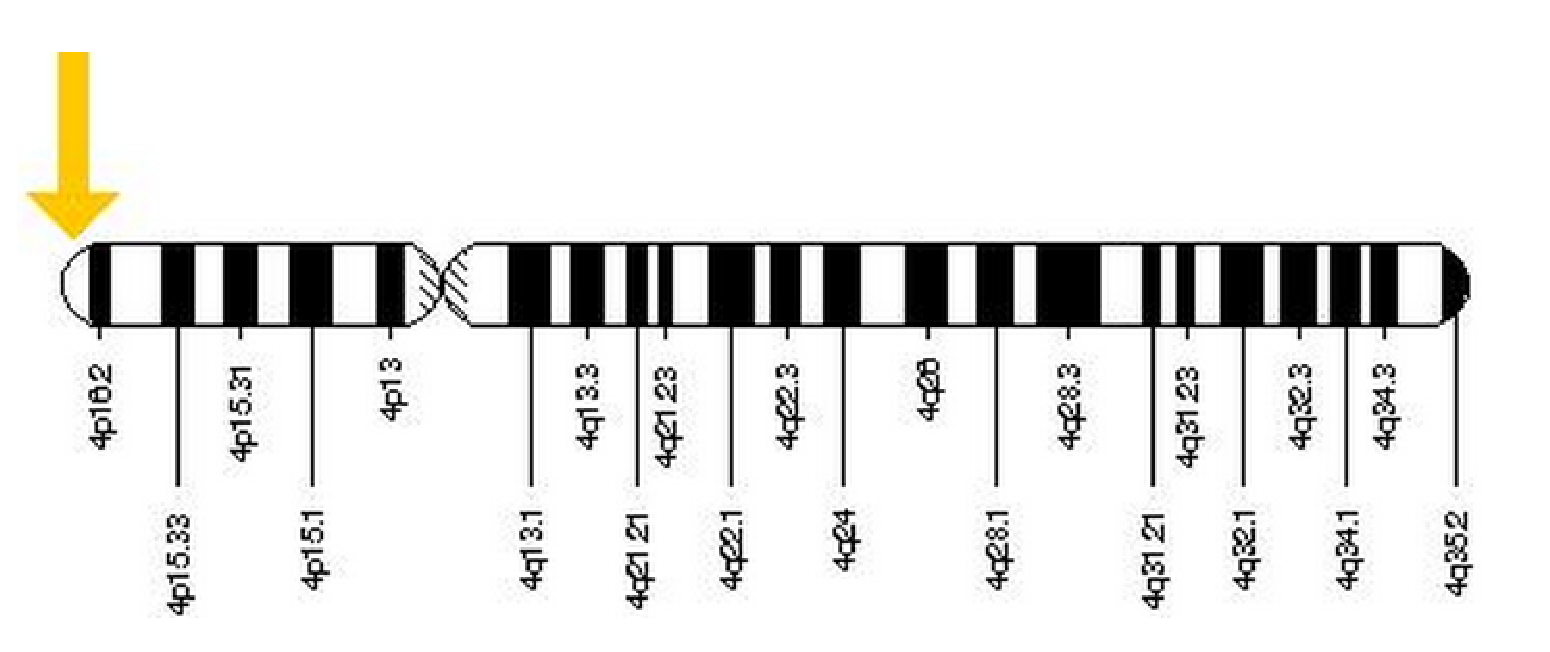
\includegraphics[height=6cm]{./images/chromosome.eps}}
  \caption{HTT gene locates on {\bf chromosome 4 (location 4p16.3}, i.e. short
  (p) arm of chromosome 4 at position 16.3, precisely from base pair 3,074,509
  to base pair 3,243,959). There are total 24 chromosomes in human (naming from
  1 to 22, and two sex chromosomes X + Y) and chromosome 4 contains 1000
  genes}\label{fig:chromosome_4}
% http://ghr.nlm.nih.gov/gene/HTT
\end{figure}

\subsection{mHTT gene (in exon-1) and mHtt protein: }
\label{sec:mHtt-protein}
\label{sec:mHTT-gene}
%\section{Types and Prevalances}
\label{sec:HD-types}

The genetic cause of HD (Sect.\ref{sec:HD-phenotype}) was discovered in 1993 -
the HD Collaborative Research Group reported that HTT mutation caused by
abnormal high number of repetition of CAG triplet at exon-1 only
\citep{HDgroup1993}; leading to the expanded poly-glutamine tract (i.e. poly-Q
or polyQ)  in the N-terminus of of the expressed Htt protein, i.e.
(Sect.\ref{sec:pathogenesis-Huntington}). NOTE: Glutamine (Q) is encoded by CAG
triplet.

The unstable expansion of CAG repeat in {\bf exon 1} of the HTT gene is the
reason for mutated Htt protein . This CAG repreat expansion
(Sect.\ref{sec:CAG-expansion}) is a type of DNA-triplets expansion
(Sect.\ref{sec:trinucleotide-expansion}).
Huntingtin (Htt) is the largest of the polyglutamine disease proteins known to
date, consisting of 3144 amno acids (MacDonald 2003).

A normal HTT gene (Sect.\ref{sec:HTT_gene}) has about 3-30 CAG triplet repeats
on exon 1. Some papers say wild-type chromosomes with a stable CAG repeat have
6-34 repeat units; more than 36 repeats results in an unstable, expanded,
disease-causing allele.



% The mutated Htt protein is the product of a mutated HTT gene
% , causing a stretch of  expanded polyglutamine (i.e.
% long polyQ of \textcolor{red}{>40 glutamines}) in exon 1.

% \begin{mdframed}
% 
% CAG repeat encodes an expanded in the huntingtin
% protein. In normal gene, there are about 10-35 repeats of CAG.
% An increase to 35-120 repeats of CAG segment can lead to the production of an
% abnormally long version of the huntingtin protein that triggers Huntington
% disease.
% \url{http://en.wikipedia.org/wiki/Trinucleotide_repeat_disorder}
% 
% \end{mdframed}


\section{Htt protein}
\label{sec:Htt-protein}

Human HTT gene (Sect.\ref{sec:HTT_gene}) provides instructions for making an
unusually large 3,144 amino-acid ($\tilde{}$ 350 kDa, or, to be exact, 348 kDa)
protein called {\bf huntingtin} (HTT) whose cellular function is still under
investigation even after 30 years (Sect.\ref{sec:protein-length}). 

The typical length of a protein is discussed in Sect.\ref{sec:protein-length}.
HTT is a very large protein (3144 a.a. in human; 3120 a.a. in mouse) which is
predicted to consist mainly (about 36) of repeated units called
\textcolor{red}{HEAT repeat domain} (Sect.\ref{sec:HEAT-repeat}) (Takano \&
Gusella 2002) - hydrophobic $\alpha$-helices that mediate
protein-protein interactions - spanning from amino acids 90 to 3144, suggesting
that huntingtin is a multifunctional scaffold protein (Andrade \& Bork 1995).

\subsection{Localization}
\label{sec:HTT-protein-localization}

Considering the expression of Htt protein, we aim to answer
\begin{enumerate}
  \item in what brain regions?
  \item distribution within an individual cell of that region?
\end{enumerate}

\subsection{-- (body/brain region) localization}

The Htt protein is expressed present in all the cells of the body, not just
nerve cells, though with different relative abundance in various fetal and adult
tissues. Htt protein seems to be necessary for development and is active
throughout the body, i.e. lacking Htt protein causes birth deffect.

Htt is expressed from early embryogenesis throughout the organism's life.
It is widely expressed in the CNS (in both neuronal and non-neuronal cell types)
and peripheral tissues (indeed the whole body) (Bhide et al. 1996, Li et al.
1993, Strong et al. 1993) (DiFiglia et al. 1995,
Gutekunst et al. 1995, Sharp et al. 1995).

\subsection{-- (subcellular) localization}

QUESTION: 
\begin{enumerate}
  \item Is it more in cytoplasm or more in nucleus, or the same?
  \item Is it more in the soma, or axon or dendrite?
\end{enumerate}

Endogenous HTT has been detected and localised in various cell lines and in
human, mouse, rat, rabbit and monkey tissue, using various antibodies, with both
cytoplasmic and nuclear localisation of HTT. However, the results are still
controversial (Hughes, Jones, 2011).
\begin{itemize}

  \item  nuclear localisation was more prominent when cross-linking fixation
  methods were used, and diminished when more dehydrating methods were employed 
  
  \item 
\end{itemize}

It is suggested that immunostaining patterns should be interpreted with caution
and related closely to the methodology employed where a lack of consistency is
found between studies.

The antibodies (- Sect.\ref{sec:antibody}) employed in these studies have
spanned the entire length of the HTT protein (as shown in Table 1) thus
indicating that the nuclear and cytoplasmic immunostaining seen does not appear
to correspond to any particular HTT fragment, but rather the full length
protein, or possibly a mixture of fragments.


Huntingtin is enriched in the subcellular fraction containing vesicle-associated
proteins (DiFiglia et al. 1995) and is transported by anterograde and retrograde
axonal transport in rat sciatic nerve (Block-Galarza et al. 1997).



\subsection{Function}
\label{sec:Htt-protein-function}

As the protein does not display significant homology to any other known
proteins, and \textcolor{red}{importantly, Htt protein also undergoes extensive
post-translational modification} (Sect.\ref{sec:Htt-PTM}), it makes harder to
predict the function (Sect.\ref{sec:Htt-protein-function}); though it seems
that the presence of the Htt protein is vital.

The essential role of htt in mammalian development was established using
constitutive HD knockout mice (Duyao et al. 1995, Nasir et al. 1995, Zeitlin et
al. 1995). Both forms of studies argue that wild-type htt has a crucial role in
cell viability.

This is described from old to newer evidences:
\begin{enumerate}
  \item \textcolor{red}{beneficial activities:  Htt possesses antiapoptotic
  properties.}

EVIDENCE: Mice lacking htt (Zeitlin et al., 1995) showed an increase programmed
cell death during development. In mice, the absence of htt causes cell
degeneration and embryonic  lethality.

EVIDENCE: conditional knockout mice show degeneration in adult neurons
(Dragatsis et al. 2000). 

This property is also showed to be beneficial/important in adults, as late
inactivation of htt in a conditional mouse model leads to progressive
neurodenegeration (Dragatsis et al., 2000).
  
  \item \textcolor{red}{beneficial activities: intracellular trafficking of
  molecules} (mitochondria, BDNF) via fast-axonal transport (Gunawardena et al., 2003; Szebenyi et al., 2003)

EVIDENCE: Htt interacts with HAP-1 protein (Sect.\ref{sec:HAP1}) which interact
with p150$^\text{Glued}$. htt could participate in the vesicular transport. So,
WT Htt helps to up-regulate BDNF. 

In HD: potential loss-of-(beneficial)function:
potential deffect in BDNF delivery
(Sect.\ref{sec:HD-theory-BDNF-impaired-transport}), or Mitochondria transport
(Sect.\ref{sec:HD-theory-mitochondria}) in HD.

\end{enumerate}

\subsection{-- role of polyQ}

It seems that the presence of poly-Q in Htt protein is not important for normal
function; as mouse htt has 7 glutamines and pufferfish htt contains only 4
(Harjes \& Wanker 2003). In addition, deletion of the CAG repeat from the mouse
HD gene results in only subtle behavioral and motor phenotypes (Clabough \&
Zeitlin 2006).




\subsection{-- Htt post-translational modification (PTM)}
\label{sec:Htt-PTM}
\label{sec:Htt-Post-translational-modification}

Glutamine (Q) 

\subsection{-- Phosphorylation of Htt}
\label{sec:mHtt-phosphorylation}

Phosphorylation has been shown to have a significant impact on expanded
huntingtin-mediated cellular toxicity.
Huntingtin phosphorylation acts as a molecular switch for anterograde/retrograde
transport in neurons (Sect.\ref{sec:fast-axonal-transport}).

Several phosphorylation sites have been identified on the huntingtin (Htt)
protein.

\begin{enumerate}
  \item pS421 site (Ser421) - Sect.\ref{sec:HD-theory-BDNF-impaired-transport}

When Htt is phosphorylated at Serine 421 (pS421Htt), anterograde transport is
facilitated, and in the presence of absent or reduced phosphorylation at this
site, retrograde transport is favored. The effect on transport is tested for
BDNF (Colin et al., 2008), but also applies to other vesicles suggesting an
essential role for huntingtin in the control of vesicular directionality in
neurons. The reduced phosphorylation at S421 of mHtt, leading to retrograde
transport, rather than anterograde transport of mitochondria (Zala et al., 2008).
% Zala D, Colin E, Rangone H, Liot G, Humbert S, Saudou F. Phosphorylation of
% mutant huntingtin at S421 restores anterograde and retrograde transport in
% neurons. Hum Mol Genet. 2008;17:3837-3846

The phosphorylation at S421 is dependent upon Manganese concentration.
Manganese (Mn) also affect phosphorylation, i.e. alter function of Htt.
Mn-exposed hippocampal and cortical primary neurons. Mn exposure significantly
reduced pS421-Htt levels. There is an apparent increase in total Htt (tHtt)
protein at the highest level of Mn exposure (5 $\muM$); though it has  no effect at 1
$\muM$ Mn in hippocampal neurons.

NMDA excitoticity stimulus leads to dephosphorylation of Ser421Htt. The
mechanism is suggested via PP1 and PP2A as blocking PP1 and PP2A activity
protects YAC128 striatal neurons from NMDA-induced cell death (Metzler,
et al., 2010 - Hayden group).

  
IGF-1/Akt pathway can compenstate for the transport defect by promoting mHtt
phosphorylation (Zala et al., 2008).

  
  \item S116A site: that had a protective effect against expanded
  polyglutamine-mediated cellular toxicity (Watkin et al., 2014)
%Phosphorylation of Mutant Huntingtin at Serine 116 Modulates Neuronal Toxicity  
  
The novel phosphorylation sites on N-terminal Htt was identified using 
exon-1 expressed in HEK293 cells.

  
\end{enumerate}


\subsection{-- Htt-protein interaction}
\label{sec:HTT-protein-interaction}

Given the large size of Htt and its repeated 36 HEAT domains
(Sect.\ref{sec:HEAT-repeat}), it is not surprising that this protein seems to
interact with a variety of cellular proteins involved in many pathways
(MacDonald 2003).

A huntingtinprotein interaction network revealed a large number of proteins
(186) that interact directly with huntingtin using yeast two-hybrid assays
(Goehler et al. 2004).


Two transcriptional pathways are more extensively implicated in HD: the
Cre-binding protein (CBP)/p300 and Sp1 pathways. 


\section{Phenotype: stages of diseases}
\label{sec:HD-phenotype}

HD impacts individual and social performance mainly through impaired cognitive,
affective and motor function. However, the cellular mechanism of disease
progression is not fully understand due to (1) slow progression of the disease,
(2) wide range of observed deffects in the CNS (Sect.\ref{sec:HD-challenge}).

Mouse model is often being used to study the mechanism and theurapeutic
development, but it is not clear if human and mouse goes through the same
mechanisms (Sect.\ref{sec:HD-mouse-models}) due to the differene in disease
progression rate.

\subsection{Age of onset: types and prevalances}

However, the two types (to be discussed below) seem start with dysfunciton in
two different pathways (Sect.\ref{sec:HD-theory-cortical-input}).

The age of onset correlates inversely with the length of the CAG
tracts with alleles $\ge$ 70 causing juvenile-onset disease
(Sect.\ref{sec:mHTT-gene}).
In the range
\begin{itemize}
  
  \item 27-35 repeats of CAG in HTT gene: individuals do not develop
Huntington disease, but they are at risk of having children who will develop the
disorder. 

As the gene is passed from parent to child (Sect.\ref{sec:genetics_Huntington}),
the number of repeats can increases into the range associated with Huntington
disease (36 repeats or more).

  \item 36-39 CAG repeats: individuals may or may not develop the signs and
  symptoms of Huntington disease

  \item >39 CAG repeats: patients develop full penetrance, i.e. almost
  always develop the disorder by age 65 years; and show first sign of HD at
  35-40 years of age (Sect.\ref{sec:HD-adult}).
  
  \item 50-200 CAG repeats (the highest number reported): may precipitate HD
  onset in childhood HD or teenage years (Sect.\ref{sec:HD-Juvenile}).
\end{itemize}   


\begin{enumerate}
  \item  The most common form is Adult-onset Huntington disease (appears in a
  person's 30s or 40s). 

The typical age of onset in between 35-50 years old (i.e. mean age of onset is
40 years), with death occurring 15-20 years from onset.
  
  \item A less common form is juvenile form HD that begins in childhood or
  adolescence. 
  
Juvenile Huntington disease: 15\% of patients.
\end{enumerate}

\subsection{-- Adult-onset HD}
\label{sec:HD-adult}

Individuals with the adult-onset form of Huntington disease usually live about
15 to 20 years after signs and symptoms begin. 

HD symptoms typically become noticeable in middle age, affecting about 1 in
every 10,000-20,000 people in the United States (Harper, 1992; Paradisi et al.,
2008). It is estimated 3 to 7 per 100,000 people of European ancestry. The
disorder appears to be less common in some other populations, including people
of Japanese, Chinese, and African descent.

\subsection{------ stages}

{\bf Neuronal loss} or {\bf neuronal dysfunction} also leads to cognitive
problems, behavioral abnormalities, and psychological dysfunction, some of which
are reported before motor abnormalities are noticeable

In adult-onset HD, patients shows a progressive deterioration of motor and
cognitive function in 3 well-defined stages.

\begin{enumerate}
  \item Stage 1: apathy, irritability, depression, and other
  mood alterations (Harper, 1991; Reedeker et al., 2012; Thompson et al., 2012).
  
  Slight motor abnormalities, such as motortics and jerky  
  voluntary movements, also are likely (Beste et al.,2009).

  \item Stage 2: dramatic increase in voluntary movements, which become
  generalized, abrupt, and uncontrolled (i.e. choreic movements -
  Sect.\ref{sec:chorea})
  
  Cognitive capacities progressively decline and finally culminate in dementia.
  Another hallmark of stage 2 is the loss of body weight despite efforts to
  maintain a high caloric diet (Marder et al., 2009)
  
  \item Stage 3 (typically occur at 10-15 years after the diagnosis):
  choreic movements are replaced by bradykinesia, and rigidity.
  
  Death becomes imminent, and the most common cause of death at this stage is
  pneumonia and heart diseases.
   
\end{enumerate}

\subsection{-- Juvenile-HD}
\label{sec:HD-Juvenile}

Juvenile Huntington's disease (JHD)  is relatively rare and accounts for
approximately 3-10\% of all patients, was first provided by Lyon in 1863 (Lyon,
1863), a few years before George Huntington described the disease that bears his
name. Prevalence estimates by one UK study cited an annual average prevalence of
juvenile HD between 1990 and 2010 as 6.77/million (95\% CI 5.60 to 8.12/million) 


JHD is defined as disease onset before age 21, with childhood disease defined as
onset before age 10 (often characterized by greater than 60 CAG repeats
(Quarrell, Strong, 2012), although occasionally as few as 45 can be encountered
(Telenius et al., 1993; Langbehn and Paulsen, 2007). It is very rare for JHD to
present before 10 years of age, though cases, including disease presentation at
18 months of age, have been reported in the literature (Nicholas et al., 2011).

% Quarrell O, O'Donovan KL, Bandmann O, Strong M. The prevalence of juvenile
% Huntington's disease: a review of the literature and meta-analysis. PLos Curr.
% 2012;4:e4f8606b742ef3.

% Nicholas G, Devys D, Goldenberg A, Maltete D, Herve C, Hannequin D,
% Guyant-Marechal L. Juvenile Huntington disease in a 18-month-old boy revealed by
% global developmental dealy and reduced cerebellar volume. Am J Med Genet
% 2011;Part A 155:815-818.  

Rigidity is the distinguishing feature of JHD in contrast with adult-onset HD.
Dystonia and epilepsy are also more common in JHD than adult HD (Quigley, 2017).
Motor symptoms in juvenile HD are more often tremor, bradykinesia, and dystonia,
rather than the chorea seen classically in adult HD. 
% Juvenile-onset patients show bradykinesia, rigidity, epilepsy, severe dementia,
% and a more rapidly progressing disease. 
Motor symptoms in juvenile HD are more often tremor, bradykinesia, and dystonia,
rather than the chorea seen classically in adult HD. 

Juvenile Huntington disease tends to progress more quickly than the adult-onset
form; affected individuals usually live 10 to 15 years after signs and symptoms
appear. 


\subsection{------ stages }


The literature cites three general stages of JHD: 
\begin{enumerate}
  \item Stage 1: behavioral disruption, learning impairments, gait changes and
  mild chorea 

The most frequent symptoms at disease onset involve developmental
delay (e.g. speech delay), cognitive dysfunction and a behavioral disorder
(where primary attention deficit hyperactivity disorder).

Early onset cases of HD most often show loss of cerebellar Purkinje cells
(Vonsattel and DiFiglia 1998), along with generalized atrophy of the brain -
Sect.\ref{sec:HD-theory-cerebellar-Purkinje-cell}

 
  \item Stage 2: rapid cognitive changes, rigidity, speech deficits and seizures

Once the disease progresses, oropharyngeal dysfunction and more
dysfunction of 'typical' motor features become more prominent, including
dystonia, rigidity, chorea, and upper motor neuron signs
  
  \item Stage 3: hypotonia, increase in seizure activity and immobility
\end{enumerate}
   

\subsection{Early signs and symptoms (chorea)}
\label{sec:chorea}

HD is a devastating neurodegenerative disorder that affects muscle coordination
and leads to gradual cognitive decline and dementia; there are currently no
effective treatments available. HD causes uncontrolled movements (choreic
movement), emotional problems, and loss of thinking ability (cognition).
{\bf Chorea} is characterized by brief, irregular contractions that are not
repetitive or rhythmic, but appear to flow from one muscle to the next. 
Chorea often occurs with athetosis, which adds twisting and writhing movements

Early signs and symptoms can include irritability, depression, small involuntary
movements, poor coordination, and trouble learning new information or making
decisions. Many people with Huntington disease develop involuntary jerking or
twitching movements known as chorea. Affected individuals may have trouble
walking, speaking, and swallowing. People with this disorder also experience
changes in personality and a decline in thinking and reasoning abilities.
Additional signs of the juvenile form include slow movements, clumsiness,
frequent falling, rigidity, slurred speech, and drooling.

%\section{Consequence}

% Clinical features of HD can be divided into three groups: (1) movement
% disorders, (2) cognitive impairment, and (3) psychiatric manifestations.


The main clinical manifestations of HD can be divided into 3 groups:
\begin{enumerate}
  \item chorea: neurological disorder characterized by jerky involuntary
  movements which appear unpredictably in all the parts of the body, 
  especially the shoulders, hips, and face (Quinn and Schrag, 1998).
  
  This is the most characteristic movement disorder of classical HD.
  Contrary to patients with typical HD, those with the juvenile form (or the
  Westphal variant) do not display chorea.
  
  As the disease progresses, the choreic movements generally tend to diminish
  and be replaced by akineto-rigid parkinsonism that can be associated with
  dystonic postures  (Penney et al., 1990; Kremer et al., 1992).
  
  \item cognitive impairment: plays a major role in the functional decline and
  loss of autonomy of the patients. 
  
  It usually leads, in turn, to dementia.
  Instrumental functions (language, praxia, and gnosis) and {\bf memory} are
  generally better preserved in HD than in other types of dementia (Caine et
  al., 1977; Hodges et al., 1990; Pillon et al., 1993, 1994).
  
  \item psychiatric disorders:
  
  Irritability, agitation, apathy, anxiety, social withdrawal, impulsiveness,
  alcohol abuse, obsessive-compulsive disorder (Cummings and Cunningham, 1992;
  Patzold and Brune, 2002), hostility, and sexual disorders are common (Pflanz
  et al., 1991; Fedoroff et al., 1994; Paulsen et al., 2001). Mood disorders are
  very frequent along HD, including depression (Caine and Shoulson, 1983;
  Folstein et al., 1983; Di Maio et al., 1993; Cummings, 1995; Jensen et al.,
  1998) and manic episodes (Mendez, 2000). Various types of psychotic disorders
  can also be observed (Cummings, 1995; Rosenblatt and Leroi, 2000). HD patients
  have a risk of suicide that is 10 times higher than in the general population.
  Sleep disorders and weight loss are also frequently encountered in HD patients
  (Morton et al., 2005; Arnulf et al., 2008; Aziz et al., 2008; Videnovic et
  al., 2009).
\end{enumerate}


In juvenile HD, school performance declines as thinking and reasoning abilities
become impaired. Seizures occur in 30 percent to 50 percent of children with
this condition. These forms are characterized by a combination of progressive
akineto-rigid parkinsonism, dystonia, ataxia, dementia, and psychiatric
disorders (Siesling et al., 1997; Gonzalez-Alegre and Afifi, 2006). Seizures can
also occur. Patients with childhood-onset HD can develop non-specific
encephalopathy resulting in seizures, myoclonus, and rapid cognitive
deterioration (Siesling et al., 1997; Gambardella et al., 2001; Gonzalez-Alegre
and Afifi, 2006).




\subsection{Brain damage}


In [adult onset] HD patients, it starts with hyperkinetic motor symptoms; while
in contrast, hypokinesic behaviors are the predominant feature of juvenile HD
(JHD) (Letort and Gonzalez-Alegre, 2013), ascribed to 'striatal failure', when
both pathways (IP and DP) are affected -
Sect.\ref{sec:HD-theory-cortical-input}.

\begin{enumerate}
  \item Adult-HD ({\bf hyperkinetic motor symptoms}):

  
A hypothesis to explain the hyperkinetic motor symptoms of [adult onset] HD
patients: a reduction in iSPN output and disinhibition of GPe would lead to
reduced subthalamic nucleus (STN) activity, diminished inhibition of motor
thalamus and 4 impairment of motor control generated through aberrant motor
cortex output. As the direct pathway (DP) becomes compromised later in disease
pathology, a difficulty in initiating movements emerges, where characteristic
bradykinesia and dystonic symptoms occur (Reedeker et al., 2010).

  \item Juvenile-HD ({\bf hypokinetic motor symptoms}): Sect.\ref{sec:HD-types}
  
All HD preclinical rodent models carry CAG repeat expansions within or extending
JHD CAG lengths (>50) and are predominantly hypokinetic (reviewed in Plotkin and
Surmeier, 2015). Thus, HD rodent models may better represent JHD, displaying
concurrent IP and DP dysfunction.

\end{enumerate}

The mHtt protein (Sect.\ref{sec:pathogenesis-Huntington}) only
selectively kills nerve cells (but not cells in other parts of the body).
Through the studies of transgenic HD animal model and postmortem HD brains of
human patients, it revealed that although mutant Htt protein is ubiquitously
expressed, the most prominent pathology occurs in cerebral cortex and striatum
(particularly the striatum (Sect.\ref{sec:basal-ganglia})), although
exactly how is not yet fully understood.



The memory decline symptoms, especially those affecting short-term memory
(Sect.\ref{sec:short-term_memory}), typically appear before any motor function
symptoms. As the disease progresses, memory deficits tend to appear, ranging
from short-term to long-term memory difficulties
(Sect.\ref{sec:long-term_memory}), including deficits in episodic, procedural
and working memory, ultimately leading to dementia.
Memory is affected by damage to the important brain pathways that help the inner
{\bf subcortical} and {\bf prefrontal} cortex, mainly in the {\bf striatum}
(Sect.\ref{sec:striatum}).
It causes selective death of the {\bf medium-sized spiny neurons (MSN, aka
striatal projection neurons (SPN))} (Sect.\ref{sec:medium_spiny_neurons})
(i.e. striatal atrophy) in the neostriatum, resulting in the appearance of
generalized involuntary movements, the main phenotypic alteration of HD.

Striatal atrophy (i.e. degrade in striatum neurons) begins as early as 15 years
before disease onset and continues throughout the period of manifest illness.
Therefore, patients could theoretically benefit from therapy at early stages of
the disease. Huntington's disease is also emerging as a model for strategies to
develop therapeutic interventions, not only to slow progression of manifest disease but
also to delay, or ideally prevent, its onset.
The reason is that {\it Huntington disease is monogenic, fully
penetrant, and} - similar to other neurodegenerative
diseases - {\it a disorder of protein misfolding}.

Within the brain, there is massive striatal neuronal cell death, with up to 95\%
loss of {\bf GABAergic medium spiny projection neurons} (MSN)
(Sect.\ref{sec:medium_spiny_neurons}) as it is the major neurons in the
striatum, which project to the globus pallidus and the substantia nigra, whereas
large interneurons are selectively spared.

\textcolor{red}{Within regionso of caudate, dorsal regions demonstrating more
decreases of these mRNA species, affecting the striosomal compartment first}
(Hedreen and Folstein, 1995; Augood et al. (1996).
% J.C. Hedreen, S.E. Folstein
% Early loss of neostriatal striosome neurons in Huntington's disease
% J. Neuropathol. Exp. Neurol., 54 (1995), pp. 105-120
% S.J. Augood, R.L.M. Faull, D.R. Love, P.C. Emson
% Reduction in enkephalin and substance P messenger RNA in the striatum of early
% grade Huntington's disease: a detailed cellular in situ hybridization study 



\subsection{-- brain atrophy}




\section{HIGHEST LEVEL THEORIES}
\label{sec:HD-theory-common-ground}

This refers to the common-ground hypothesis (i.e. most abstract level), and any
other hypothesis are derived based upon
\begin{enumerate}
  \item {\bf defect in the CNS}: 
  
The progressive cognitive, affective and motor dysfunction in Huntington's
disease (HD) result from progressive pathophysiology of the central nervous
system.

  \item {\bf caused by mHtt}:
  
The failure above is derived from a mutation in the huntingtin gene (mHTT) in
the form of an expansion in the number of repeats in the CAG triplet (>37) in
exon 1 and from the resultant protein (mHTT) with its corresponding expanded
polyglutamine tract (>37 residues).

This could be gain-of-function (i.e. gain of new toxic function of WT Htt)
and/or loss-of-function (i.e. loss of beneficial activities of WT Htt) -
(Cattaneo et al., 2001; Ross, 2002)..


\end{enumerate}

Common principles in efforts in studying neural functions and dysfunctions is
discussed in Sect.\ref{sec:brain-disease-circuit-level}.

\section{Challenges}
\label{sec:HD-challenge}

Given the widely adopted hypothesis discussed in
Sect.\ref{sec:HD-theory-common-ground}, finding which changes is {\bf causal}
(i.e. primary); which changes is {\bf adaptive} (i.e. secondary) is challenging. 

From post-moterm analysis, striatum is found to be the major brain region
affected, early hypothesis was focusing on striatal dysfunction or more lately,
cortico-striatal pathology is considered flawed or oversimplified
(Sect.\ref{sec:HD-theory-flawed-theories}). However, such focus on the
importance of extra-striatal dysfunction and degeneration (in particular
cortical degeneration and corticostriatal projection loss) has improved our
understanding of the progress of disease pathology, although this has yet to be
conceptually framed within a cohesive theory of how CNS dysfunction progresses
in HD.

This requires
\begin{enumerate}
  \item understanding dynamics of BG macrocircuit -
  Sect.\ref{sec:HD-theory-BG-macrocircuit}

It needs a fundamental characterization of the cortico-striato-thalamocortical
macrocircuit in HD [and HD models] -
Sect.\ref{sec:cortico-striato-thalamo-cortical-pathway}; and it needs a
conceptualization of how that circuitry dysfunction drives symptomatology.
    
  \item targeting the most proximal cause - lowering mHtt protein -
  Sect.\ref{sec:HD-theory-lowering-mHtt}
  
  \item 
\end{enumerate}

Based on CHDI's white paper, the advances in understanding of 'normal'
cortico-basal ganglia macrocircuitry and information processing advance, though
is good, is not yet adequately applied to updated theories of the emanation of
circuitry dysfunction in HD, nor its correlation to 'conversion', disease
progression and symptom presentation.

% While advances in understanding of 'normal' cortico-basal ganglia macrocircuitry
% and information processing advance, this is not yet adequately applied to
% updated theories of the emanation of circuitry dysfunction in HD, nor its
% correlation to 'conversion', disease progression and symptom presentation.

This is in part due to the lack of definitive models of how normal behaviors
such as volitional movements, ordered thoughts, or general affect arise from
their neural substrates.

\subsection{When the HD disease is really 'initiated' (new born, early child,
adult)?}

Htt is shown to be essential for embryonic development and neurogenesis (White
et al., 1997; Zeitlin et al., 1995).

Diseases caused by mHtt could be gain-of-function (i.e. gain of new toxic
function of WT Htt) and/or loss-of-function (i.e. loss of beneficial activities
of WT Htt) - (Cattaneo et al., 2001; Ross, 2002) -
Sect.\ref{sec:Htt-protein-function}.

Based on the finding that reduced mRNA level of certain genes
(Sect.\ref{sec:HD-theory-transcription-dysfunction}), one could argue that
decreases in mRNA encoding neurotransmitter receptors were a developmental
effect, as the mutant transgene is expressed throughout development.
However, the observation that young R6/2 mice were phenotypically
indistinguishable from wild-type littermates argues against the notion of a
developmental defect.

\subsection{-- where in the brain is initiated first (i.e. observable)?}

The earliest signs of pathology in HD are in the striatum (Menalled and
Chesselet, 2002; Raymond et al., 2011), a subcortical structure involved in the
control of movement and action selection (Gerfen and Surmeier, 2011) -
Sect.\ref{sec:striatum}).

Two possible mechanisms to explain unwanted movements:
\begin{enumerate}
  \item unwanted trigger 
  \item failed to suppress - this is confirmed to be failure 
\end{enumerate}
In particular, there is a deficit in the ability of cortical circuits to drive
iSPNs - Sect.\ref{sec:iSPN-vs-dSPN} - has long been hypothesized to underlie
unwanted movement in the early stages of HD (Zuccato et al., 2010).

There are two things we are interested:
\begin{enumerate}
  \item why iSPN; but not dSPN?
  
  \item what deficit in iSPN?
  \begin{itemize}
    \item lack of incoming signal? - from other input neurons
    
    \item signal is normal, but failure to response? - from internal of the
    iSPN.
  \end{itemize}
\end{enumerate}


\subsection{Is persistent presence of mHtt required for the HD progression?}

\subsection{-- if not, at what point it is no longer required?}

\subsection{At what point, the brain circuitry dysfunction is IRreversible (no
matter what mHtt level)?}

\subsection{Does mHtt cause a sequential series of changes or multitudes of
changes in parallel?}

Vahri: 'Does the disease progress as a linear series of disruptions to a small,
discreet number of (cellular) morphological and physiological mechanisms, or
does mHTT loss/gain of function cause a radiation of untold multitudes of same
in parallel?'

From a therapeutics standpoint, we hope for the former but must plan for the
latter.

\subsection{What causes the symptoms?}



\section{LATE-PHASE OBSERVATION (or flawed hypothesis)}
%\section{FLAWED theories/hypothesis}
\label{sec:HD-theory-flawed-theories}

Fundamental revisions to our understanding of this macrocircuitry and
information flow through the BG have occurred in the last decades, and this,
coupled with the greater understanding of regional atrophy [and its correlation
to] heterogeneous symptom presentation in HD patients in recent years, make {\it
simplified theories of HD as primarily being driven by striatal (or more
latterly corticostriatal pathology); or due to easily defined discrete
pathophysiological processes}, highly oversimplified, if not fundamentally
flawed.

For the past decade, the striatal pathology in HD has been attributed to a
decrease in cortical BDNF delivery (Gauthier et al., 2004; Zhang et al., 2003;
Zuccato et al., 2001; Zuccato and Cattaneo, 2007). Although it does not exclude
the possibility that, later in the progression of the disease, such trafficking
deficits manifest themselves, the recent work by Surmier (Plotkin et al., 2014)
argued that deficits in TrkBR and p75NTR signaling precede them -
Sect.\ref{sec:HD-theory-impaired-TrkBR-signaling}.
There was no change in BDNF mRNA levels
(Sect.\ref{sec:mRNA-level-2-protein-expression}) in cerebral cortex of BACHD and
heterozygous Q175 HD models. The phosphorylation of striatal TrkBRs in response
to depolarization-induced release of BDNF by cortical terminals was normal in
tissue from BACHD mice.

\subsection{transcriptional dysregulation (1996+)}
\label{sec:HD-theory-transcription-dysfunction}

Even though there are clear evidence of selective neuronal susceptibility in HD,
the susceptibility here applies not to the phenomenon of cell death but of
downregulation of target genes.
It is suggested that there were regional- or cell-specific decreases in
expression of these important signaling molecules.

Even though wild-type huntingtin is predominantly a cytoplasmic protein, it is
possible that small amounts of full-length protein or proteolytically cleaved
fragments are localized in the nucleus.

4-week-old transgenic mice start off with nearly normal levels of
neurotransmitter mRNA, with levels decreasing when measured at 8 or 12 weeks of
age (Cha et al., 1999).
NOTICE: Normal mice only has only 6-7 CAG repeats
(Sect.\ref{sec:HTT-gene-Hdh-mouse}). Transgenic mice expressing exon 1 of the
human HD gene with 18 CAG repeats did not show any significant changes in
neurotransmitters.

\begin{enumerate}
  
  \item Once getting into the nucleus (where the transcription occurs), mHtt
  fragments may affect the expression level of other proteins (e.g.
  neurotransmitter receptor genes, intracellular signalling proteins, and
  calcium homeostasis) (Cha, 2000).
% https://www.ncbi.nlm.nih.gov/pubmed/10941183

   \item Alternatively, huntingtin may act within the cytoplasm by recruiting
   transcription factors.
   
However, there are no reports of transcriptional activity of wild-type
huntingtin (Zuccato et al., 2001).

\end{enumerate}


Kumar, Vaish, Ratan (2014) proposed a unifying hypothesis emerging from these
studies, which is that HD represents the pathological disruption of
evolutionarily conserved adaptive gene programs to counteract oxidative stress,
mitochondrial dysfunction and accumulation of misfolded proteins.
It is further exacerbated by the repression of genes involved in normal synaptic
activity or growth factor signaling.

How the mutated protein expressed in the cytoplasm, end up in the nucleus?
Numerous studies suggests the protein must be cleaved in order to translocate to
the nucleus and exert their toxicity.
Proteolytic cleavage of mutant htt yields polyQ-containing N-terminal fragments
that are prone to misfolding and aggregation.
Caspase-6 is required to cleave mHtt, at amino acid 558 (see below).
This process is dependent upon
\begin{enumerate}
  \item Ser-16 phosphorylation can regualte N-terminal cleavage of mHtt; and its
  nuclear transporation

N-terminal region is the nuclear export signal (NES) - and mutation at this site
enhances nuclear accumulation.
  
  \item 
\end{enumerate}


\subsection{-- cleavages: caspase-6}
\label{sec:HD-}

Nuclear translocation is an early step in pathogenesis in a HD knock-in mouse
model (Wheeler et al. 2002). Hoever, the relationship between htt proteolysis
and pathogenesis in vivo was unknown.
\textcolor{red}{Does apoptotic pathway play a primary role in neuronal
dysfunction, or is it a secondary event that occurs in dysfunctional neuron that
can no longer tolerate toxic effect of the mutant protein?} (Cummings, Zoghbi,
2000)

The search for such proteases - the enzymes that cleave protein -
Sect.\ref{sec:protease} are {\bf caspases} (Sect.\ref{sec:caspase}).
Caspase- 3 and -6, apartyl endopeptidases, and calpain have all been implicated
in the cleavage of htt. In a recent study, the role of htt cleavage by caspase-3
and caspase-6 in disease was examined by expressing caspase-3- and caspase-6-
resistant forms of mutant htt in mice (Graham et al. 2006).
Controlling for expression levels, Graham et al. found that transgenic mice
expressing polyQ-expanded htt with a mutated caspase-6 cleavage site did not
manifest any behavioral deficits or neurodegeneration, even when the expression
level of htt exceeded that of unmutated polyglutamineexpanded htt transgenic
mice. Also, htt mutated at caspase-6 cleavage sites had a significant delay in
its nuclear translocation. In contrast, the caspase-3- resistant form of mutant
htt remained fully pathogenic. This suggest the important role of caspase-6 in
pathogenesis.

\subsection{-- decrease neuropeptide mRNA level: 1996}

Augood et al. (1996) measure messenger RNA (mRNA) encoding the signaling
neuropeptides enkephalin and substance P.


Within the caudate-putamen, there was a heterogeneous distribution of mRNA
loss, reinforcing the idea of selective neuronal susceptibility. 
The susceptibility here applies not to the phenomenon of cell death but of
downregulation of target genes. 

\subsection{-- decrease DA-receptor mRNA level (1997)}

Neurotransmitter receptors that are altered in HD (receptors for glutamate,
dopamine, acetylcholine and adenosine) are decreased in the brain of transgenic
mice, in some cases before the onset of behavioural or motor symptoms.  
Receptor decreases are preceded by selective decreases in the corresponding mRNA
species, suggesting the altered transcription of specific genes might be a key
pathological mechanism in HD
(Sect.\ref{sec:HD-theory-transcription-dysfunction})

\begin{mdframed}
Receptor binding autoradiography is a measure of the amount of receptor protein,
and \textcolor{red}{decreased protein could result from a number of mechanisms,
including disrupted trafficking or accelerated protein degradation. 
An alternate explanation was that the decreased protein levels actually
reflected a failure to generate adequate amounts of the corresponding mRNA.}

In order to discriminate between these possibilities, in R6/2 mouse, Cha et al.,
1998 ; Cha et al., 1999 measured levels of mRNA encoding neurotransmitter receptors, and
found that those receptors that had decreased proteins levels had decreased mRNA
levels as well  
\end{mdframed}

Augood et al. (1997) showed mRNA encoding dopamine D1 receptor (D1) and dopamine
D2 receptor (D2) in the caudates of HD brains of different pathological grades
\begin{itemize}
  \item  grade 0 refers to brains that have no recognizable neuropathologic
  abnormality

Decreased numbers of cell expressing the D1 mRNA; and those express do express
at a normal level (as based on the counting number of mRNA molecules per cell).

Decreased number of cell expressing the D2 mRNA; but also the
number of D2 messages per cell was decreasing. The second part is opposite to
D1-MSN. \textcolor{red}{This suggests D1-MSN and D2-MSN are both early
affected (in the sense of reduced cell counts); yet D2-MSN is more vulnerable
(in the sense reducing the capability to sense DA signal)}.
  
  \item grade 1 implies that neuropathological abnormalities are only apparent
  microscopically.
  
  
They observed increased D1 message per cell, which they attributed to a shift in
cell populations, i.e. (with MSN die) there are relatively more interneurons,
which contain high levels of D1 mRNA.
  
\end{itemize}

At just 4 weeks of age in R6/2 mice, (Cha et al., 1998) showed decreases in D1R
mRNA level (and later decreased in dopamine receptor binding), well before the
onset of behavioral and motor symptoms in these mice.
\textcolor{red}{It is important to remember that receptor downregulation was not
simply reflective of neuronal loss, since there was not widespread striatal cell
death in R6/2 mice.}

Andrews et al., (1999) showed on human using PET imaging (Sect.\ref{sec:PET})
scanning reveals decreases in dopamine D2 receptor binding potential in HD
gene-positive human subjects who are clinically asymptomatic, supporting the
notion that functional changes can occur before overt clinical symptoms develop.

\subsection{-- decreased glutmate receptor (e.g. mGluR, AMPAR, NMDAR loss):
1998}

Glutamate receptors were not all affected to the same degree.
This reduction may be part of the mechanism to comprise the abnormal level of
glutamate (Sect.\ref{sec:HD-theory-glutamate-toxicity}).

Alteration of glutamate receptor mRNA is not limited to the striatum, as the
cortex of R6/2 also demonstrates selective decreases of certain mRNA (Cha et
al., 1998 ;  Luthi-Carter et al., 2003). 


\begin{enumerate}
  
  \item Cha et al. (1998, 1999): In R6/2 mice of symptomatic 12-week,
  glutamate receptors, as well as other neurotransmitter receptors, were altered
  in a fashion that was remarkably similar to that seen in human HD
  caudate-putamen (Cha et al., 1998). 
  
    Muscarinic cholinergic receptors were also decreased,  but there was not
  difference in GABA receptor binding. 

   Decreased mRNA encoding the mGluR1, mGluR2, and mGluR3 subtypes of the
 metabotropic glutamate receptors 
  
  
% J.-H.J. Cha, C.M. Kosinski, J.A. Kerner, S.A. Alsdorf, L. Mangiarini, S.W. Davies, J.B. Penney, G.P. Bates, A.B. Young
% Altered brain neurotransmitter receptors in transgenic mice expressing a portion of an abnormal human Huntington disease gene
% Proc. Natl. Acad. Sci. U.S.A., 95 (1998), pp. 6480-6485

  Autoradiography also revealed decreases in AMPA and metabotropic glutamate
  receptors, with relative preservation of NMDA receptor binding.
   
% J.-H.J. Cha, A.S. Frey, S.A. Alsdorf, J.A. Kerner, C.M. Kosinski, L. Mangiarini,
% J.B. Penney Jr., S.W. Davies, G.P. Bates, A.B. Young Altered neurotransmitter
% receptor expression in transgenic mouse models of Huntington's disease Philos.
% Trans. R. Soc. Lond. B Biol. Sci., 354 (1999), pp. 981-989
  
  \item Young et al. (1998)
  
  loss of NMDA receptors in the caudate-putamen of HD patients resulted from
  excitotoxic cell death
  
%   A.B. Young, J.T. Greenamyre, Z. Hollingsworth, R. Albin, C. D'Amato, I. Shoulson, J.B. Penney
% NMDA receptor losses in putamen from patients with Huntington's disease
% Science, 241 (1988), pp. 981-983

  \item (Luthi-Carter et al., 2003): there was more downregulation of NMDAR in
  the hippocampus as opposed to the striatum.
  
 \textcolor{red}{This observation calls into question whether the striatum is
 uniquely affected in HD}. The less vulnerability of the hippocampus probably
 can be explained by the fact that it is actually relatively protected from
 glutamate excitotoxicity (Sect.\ref{sec:HD-theory-glutamate-toxicity}) compared
 to the striatum, and as a result manifests less atrophy.
 
 multiple levels of NMDA receptor dysregulation: reduced mRNA expression levels,
 alter receptor stoichiometry, protein phosphorylation, and receptor
 trafficking.
  
  PSD-95 and $\alpha$-actinin-2, proteins essential for anchoring NMDA
  receptors, were decreased. tyrosine-phosphorylated $\varepsilon$1 subunit,
  another determinant of NMDA receptor trafficking, in R6/2 hippocampus. 
  
% R. Luthi-Carter, B.L. Apostol, A.W. Dunah, M.M. DeJohn, L.A. Farrell, G.P.
% Bates, A.B. Young, D.G. Standaert, L.M. Thompson, J.-H.J. Cha Complex
% alteration of NMDA receptors in transgenic Huntington's disease mouse brain:
% analysis of mRNA expression levels, protein abundance, interacting proteins
% and phosphorylation Neurobiol. Dis., 14 (2003), pp. 624-636
   

  \item Dure et al. (1991):   decreased receptor binding not only to NMDA
  receptors but also to quisqualate and kainate subtypes of glutamate receptors; 
   
  Using NMDA-displaceable [3H]glutamate, [3H]glycine and [3H]MK-801 binding to
  estimate NMDAR, they showed a decrease to a similar extent (50-60\%) as
  measures of other non-NMDA ionotropic receptors ([3H]kainate and [3H]AMPA
  binding). 
  
  For metabotropic glutamate receptors; the binding was found to be decreased to
  a lesser extent (26-31\%).

  \item Arzberger et al. (1997): study on human HD brain (postmortem)
  
  mRNA encoding the NR1 and NR2B subunits were decreased in accordance with
  disease severity, as was mRNA encoding the glutamate transporter GLT1.
    
  Analyzing mRNA in human brain samples is notoriously difficult, as RNA is
  rapidly degraded, and postmortem intervals can vary widely.
\end{enumerate}

\subsection{-- decreased glutamate transporter GLT1}

Arzberger et al. (1997) showed that mRNA encoding the glutamate transporter GLT1
is decreased - Sect.\ref{sec:GLT1}).

\subsection{-- decreased CB1R}

decreases have been found in CB1 receptors 
\begin{enumerate}
  \item   (Denovan-Wright and Robertson, 2000 ;  McCaw et al., 2004): 
   in R6/1 and R6/2 
   
  \item  (Lastres-Becker et al., 2002: in HD94 mice. 
\end{enumerate}

This is similar to what had been found in (postmortem) human HD brain (Glass et
al., 1993; Glass et al., 2000 ; Richfield and Herkenham, 1994).

\subsection{-- decreased TrkB receptor}

Gines et al., 2006)  analysed the expression of TrkB in several HD models and in
postmortem HD brains; and they  found there is reduced expression of trkB, which
forms part of the cell surface receptor for BDNF.
TrkBR is reduced in
\begin{itemize}
  \item transgenic exon-1 and full-length knock-in HD mouse models and also 
  
  \item in the motor cortex and caudate nucleus of human HD brains. 
\end{itemize}
continuous expression of mutant huntingtin is required to down-regulate TrkB
levels. TrkB expression is not dependent upon the presence of BDNF

% S. Gines, M. Bosch, S. Marco, N. Gavalda, M. Diaz-Hernandez, J.J. Lucas, J.M. Canals, J. Alberch
% Reduced expression of the TrkB receptor in Huntington's disease mouse models and in human brain
% Eur. J. Neurosci., 23 (2006), pp. 649-658


\subsection{-- interneuron (survive, yet damaged in nNOS): 1996}

Norris et al. (1996) found that  interneurons of the caudate-putamen
\begin{itemize}
  \item  levels of mRNA encoding neuronal nitric oxide synthase (nNOS) -
  Sect.\ref{sec:NO-synthase}, and somatostatin were decreased on a per-cell
  basis; yet
  
  \item  neurons containing neuropeptide Y, nNOS, NADPH diaphorase, and
  somatostatin survive.
\end{itemize}
These striatal neurons survive, but are damaged, and they inferred a
progressive downregulation of nNOS messenger RNA.

\subsection{-- non-striatal brain specific region}

Kotliarova et al., (2005) found that aggregates were intense in the
hypothalamus, and decreased expression of a number of hypothalamic
neuropeptides, including oxytocin, vasopressin and cocaine-amphetamine-regulated
transcript (Kotliarova et al., 2005), indicating that transcriptional
dysregulation induced by exon 1 huntingtin can produce brain region-specific
effects, again, affecting also non-striatal regions.

% S. Kotliarova, N.R. Jana, N. Sakamoto, M. Kurosawa, H. Miyazaki, M. Nekooki, H.
% Doi, Y. Machida, H.K. Wong, T. Suzuki, C. Uchikawa, Y. Kotliarov, K. Uchida, Y.
% Nagao, U. Nagaoka, A. Tamaoka, K. Oyanagi, F. Oyama, N. Nukina Decreased
% expression of hypothalamic neuropeptides in Huntington disease transgenic mice
% with expanded polyglutamine-EGFP fluorescent aggregates J. Neurochem., 93
% (2005), pp. 641-653

\subsection{-- reduced synthatic enzyme for neurotransmitters}

Tyrosine hydroxylase is the rate-limiting enzyme for catecholamine synthesis,
and both transgenic HD mice and human HD brain demonstrate decreases in TH mRNA
(Yohrling et al., 2002). In situ hybridization revealed decreased tyrosine
hydroxylase mRNA in human HD substantia nigra neurons. In addition, mutant Htt
disrupted transcription of tyrosine hydroxylase and dopamine $\beta$-hydroxylase
promoter constructs, pointing to a direct repressive role of mutant Htt.

\subsection{intracellular Ca2+ signaling}

\subsection{-- PKC}

Harris et al. (2001) identified protein kinase C beta II as downregulated in
R6/2 mice - Sect.\ref{sec:PKC}

\subsection{-- dopaminergic system: DARPP-32}

At 4 weeks of age, the R6/2 mice displayed severe deficiencies in dopamine
signaling in the striatum.  Bibb et al. (2000) identified severe reductions of
dopamine- and cAMP-regulated phosphoprotein, M(r) 32 kDA (DARPP-32) in the
brains of R6/2 mice, as well as other dopamine-regulated phosphoprotein markers
of medium spiny neurons. van Dellen et al. (2000) identified similar decreases
in R6/1 mice.

At 6 weeks of age, the R6/2 mice resembled DARPP32 knockout mice, which also
have abnormal dopamine signaling (Greengard et al., 1999).

NOTE: Dopamine signaling is known to regulate gene transcription (Berke et al.,
1998). The DARPP-32 defect also appears to be region-specific, in that R6 mice
show decreased expression in the striatum, but normal levels in the kidney
(Gomez et al., 2006) - Sect.\ref{sec:DARPP32}. 

\subsection{structural proteins}

\subsection{-- Tenascin-C}

Tenascin-C is an extracellular matrix glycoprotein involved in cell migration,
which is downregulated in R6/2 mouse brain (Kusakabe et al., 2001).
The level is normal expression of tenascin-C in astrocytes, but reduced
expression in the cortex and thalamus.

At later ages (12 weeks), neuronal expression of tenascin-C disappeared in
several thalamic nuclei (e.g., the ventromedial, parafascicular, lateral
posterior, and posterior thalamic groups) as well as in frontal cortex.
At this age, there was an accompanying astrogliosis within the thalamus. 
\textcolor{red}{It suggests neurons are more susceptible to mRNA downregulation
than astrocytes.}
 
\subsection{-- post-synaptic: PSD-95, Citron, alpha-actinin-2}

The altered expression of postsynaptic proteins imply dysfunctional postsynaptic
responses, particularly at excitatory NMDA receptor synapses, with important
implications in terms of NMDA-receptor-mediated excitotoxicity (Jarabek et al.,
2004; Luthi-Carter et al., 2003 ;  Sun et al., 2001).

Huntingtin binds directly to PSD-95 (Sun et al., 2001), and PSD-95 levels
decreased in R6/2 mice (Luthi-Carter et al., 2003). 

Citron is a protein that binds to PSD-95 that is involved in dendritic spine
formation (Zhang et al., 1999).  Citron expression is decreased in the brains of
N171-82Q mice (Jarabek et al., 2004). 

$\alpha$-actinin-2, another glutamate receptor anchoring protein, is decreased in R6/2
mouse brain (Luthi-Carter et al., 2003).

\subsection{-- pre-synaptic:}

mHtt may disrupt neurotransmitter release by sequestering complexin II into
aggregates and rendering the presynaptic vesicles unable to release
neurotransmitter.

SNAP and complexin I are also decreased in R6/2 brain, but these changes lag
behind the decrease in complexin II.

Complexin II is a component of the SNARE complex, and is likely to be involved
in the control of exocytosis. Complexin II levels are progressively decreased in
the brains of R6/2 mice (Morton and Edwardson, 2001).
 Complexin II was also found to co-aggregate with huntingtin to form
intranuclear inclusions.

Rabphilin 3A, another protein involved in exocytosis, is decreased in the brains
of R6/2 mice (Smith et al., 2005). 

\subsection{neurotoxicity}
\label{sec:HD-theory-neuro-toxicity}

\subsection{-- aggregation}
\label{sec:mHTT-protein-aggregate}
\label{sec:HD-theory-mHTT-aggregation}

White et al. (1997) suggested that the level of Hdh protein in mouse play a
critical function in neurogenesis; by showing that HdhQ50 that expressed
wild-type level of altered Htt gene does not affect the brain; and reduced level
(HdhneoQ50) displayed characteristic aberrant brain development and perinatal
lethality.

Also, it suggested the expanded CAG repeat does not eliminate or detectably
impair huntingtin's neurogenic function. So, in HdhQ50 mouse with impaired
brain function, there should be a gain-of-function, i.e.
enhanced level of altered Htt gene.

\begin{mdframed}
\textcolor{red}{Question: mHtt leading to gain-of-function or loss-of-function
disease?} (even though the function of Htt protein is not clearly understood).

\begin{enumerate}
  \item gain-of-function hypothesis: (White et al., 1997)
  
  \item loss-of-function hypothesis: not for HD disease; but this is seems to be
  the mechanism in HDL2 (Sect.\ref{sec:HDL2})
\end{enumerate}
\end{mdframed}

The hypothesis is that during protein synthesis, the expanded CAG repeats are
translated into a series of uninterrupted glutamine amino acid
(Sect.\ref{sec:glutamine}) forming what is known as a {\bf polyglutamine} (or
"polyQ") tract. Because glutamine is a polar, or ``charged" molecule, the
overabundance of glutamine causes links to form within and between proteins.
Such polyglutamine tracts may be subject to increased aggregation
(Sect.\ref{sec:aggregation-2-neurological-disease}).

Green proposed that this poly-Q is a trans-glutamate substrate that can
cross-linked via isopeptide bonds. This event enhances glutamine-mediated
aggregation and toxicity in affected neurons. 

\subsection{-- aggregation -- in nucleus}
\label{sec:HD-theory-mHTT-aggregation-in-nucleus}

For most of polyglutamine diseases, the protein aggregates are found
predominantly in the nucleus. Early finding suggested the forming of aggregates
similar to nucleus inclusions (NI) is a common pathogenic mechanism for all
polyglutamate disorders. \textcolor{blue}{\it Abnormal substances in the nuclei
that can be observed by light microscopy are often broadly referred to as
nuclear inclusions. }

\textcolor{red}{However, this was later found wrong.} NIs are neither necessary
or sufficient to initiate polyglutamate diseases. NIs are also found in cells
that show no sign of neurodegeneration; and only found small amount (< 1\%) in
striatum; where the most neural loss occurs.

\begin{mdframed}

MISLEADING FINDING: Ubiquitin-positive protein aggregates (primarily found in
nucleus) have been reported to 7 of these polyglutamine disorders; except gene
{\it SCA6} (spinocerebellar ataxia type 6) where aggregates are cytoplasmic and
ubiquitin-negative. In neuropil of HD's brain and transgenic mice, protein
aggregate, with similar structure to nuclear inclusion (NI), also found. Such
aggregates found in dendrites, dendritic spines are far more common in HD's
brain than NI.

\end{mdframed}

However, overall, the level of NIs are higher in polyglutamine diseases.
In the nucleus, the mutant protein can affect gene expression.

\subsection{-- aggregation -- in cytoplasm}
\label{sec:HD-theory-mHTT-aggregation-in-cytoplasm}

The hypothesis about mHTT aggeregation in the cytoplasm leading to disease has
been suggested by \ldots

The data that supported this hypothesis include
\begin{itemize}
  \item  Reducing HDAC4 by using HDAC4 inhibitor
  (Sect.\ref{sec:HD-theory-HDAC-inhibitor}).
  
  ASSUME: reduced the total burden of HTT aggregates throughout the brain while
  increasing the amount of soluble HTT.
  
  \item 
  
\end{itemize}

\subsection{-- abnormal Glut level}
\label{sec:HD-theory-glutamate-toxicity}

The selective cell loss of MSN at caudate-putamen (striatum) implies a selective
neuronal vulnerability. So, neurotransmitter - namely, glutamate - could have
toxic effects if its actions were abnormally regulated.

Glutamate excitotoxicity had historically been a leading idea regarding HD
pathogenesis (Albin and Greenamyre, 1992; Beal et al., 1991; Bruyn and Stoof,
1990; Coyle and Schwarcz, 1976 ;  DiFiglia, 1990).
This is based on the observation that injection of glutamate analogues into the
striatum of rodents or primates could reproduce the pattern of neuropathological
damage seen in HD, namely death of medium spiny projection neurons with relative
sparing of interneurons.

Arzberger et al. (1997) showed that mRNA encoding the glutamate transporter GLT1
is decreased - Sect.\ref{sec:GLT1}).

\subsection{GABA level ???}
\label{sec:HD-theory-neurotransmitter}

Reynolds et al. (1999) characterized the levels of many neurotransmitters in the
R6/2  by HPLC in four brain regions, at times before and after the emergence of
a HD-like phenotype. When compared to the human postmortem findings, several
noteworthy disparities were observed.
\begin{enumerate}
  \item  Striatal GABA in the R6/2 mice was normal

 It suggests that loss of GABA-containing neurons is not an important early
  pathogenic event in the transgenic mice, and that the GABA decreases described
  in human HD are likely simply reflective of cell loss. 
  
 So, GABA loss is probably the consequence of neuronal loss, as opposed to
 being a cause of neuronal loss
  
  \item 
\end{enumerate}
NOTE: This study did not look specifically at mRNA levels of neurotransmitter
synthetic enzymes, focusing rather on measurements of the actual
neurotransmitters themselves. 



\subsection{Dopamine, and Serotonin level ???}
\label{sec:HD-theory-neurotransmitter-Dopamine}
\label{sec:HD-theory-neurotransmitter-Serotonine}

Reynolds et al. (1999) characterized the levels of many neurotransmitters in the
R6/2  by HPLC in four brain regions, at times before and after the emergence of
a HD-like phenotype.

In the striatum of 12-week-old R6/2 mice, there were significant decreases in
dopamine and serotonin.
\begin{enumerate}
  
  \item Significant drop in  striatal 5-hydoxyindolacetic acid (5-HIAA) levels,
  the major metabolite of serotonin, was seen in 4-, 8-, and 12-week-old animals
  in striatum.
  
  Similar decreases were observed at 8 and 12 weeks of age only in the
  hippocampus and brain stem of the R6/2 mice
  
  \item Norepinephrine levels were decreased only in the hippocampus and brain
  stem
  
\end{enumerate}

Hickey et al., (2000)  showed dopamine content is reduced in the R6/2 brain by
about 9 weeks of age, but long-term replacement of dopamine (chronic treatment
with laevodopa (L-DOPA)) caused short-term improvements in activity and rearing
behaviour, and abolished abnormal spontaneous hindlimb grooming; yet long-term
treatment worsened motor function in these mice. In particular, R6/2 mice also
showed an attenuated response to cocaine, indicating that DA release may be
compromised.  R6/2 mice display an age-dependent abnormal behavioural response
to (+)-methamphetamine (METH) and a dose-dependent increase in sensitivity to
METH toxicity.

% M.A. Hickey, G.P. Reynolds, A.J. Morton
% The role of dopamine in motor symptoms in the R6/2 transgenic mouse model of Huntington's disease
% J. Neurochem., 81 (2002), pp. 46-59

\subsection{BDNF}

This peptide neurotrophic factor is decreased in the brains of HD mice and human
HD brains (Zuccato et al., 2001) -
Sect.\ref{sec:HD-theory-BDNF-impaired-transport}). Striatal BDNF is actually
produced in cortical neurons and transported through cortical efferents into the
striatum.


 
 

\subsection{impaired axonal transport defect}

{\bf Early evidences}: alteration of axonal transport by polyQ-containing
proteins (Gunawardena et al., 2003; Lee et a l., 2004; Piccioni et al., 2002;
Szebenyi et al., 2003). Two possible mechanisms
\begin{enumerate}
  \item (specific to Htt): Htt involves in intracellular transport; and mHtt
  protein affect this
  
  \item (general to all polyQ-containing protein): mutated polyQ-protein causes
  axonal blockage (i.e. axonal poisoning)
\end{enumerate}

{\bf More direct evidence} linking huntingtin to axonal transport defects comes
from 
\begin{enumerate}
  
  \item  (Gunawardena et al. 2003) studies in Drosophila, where a reduction in
  the expression of Drosophila huntingtin resulted in defects in larval neuronal transport and
neurodegeneration in adult fly eyes.

  \item (Gauthier et al. 2004) tested with {\it Hdh}$^{Q111}$ knock-in
  mouse, reported that fulllength wild-type huntingtin promotes vesicular
  transport of BDNF-containing vesicles along microtubules.
  
mHtt-induced reduction in BDNF-containing vesicle transport reduces trophic
support, causing neurotoxicity, which may contribute to pathogenesis.

\end{enumerate}


\subsection{-- impaired BDNF production or transport to axonal terminal (in
cortical neurons): pS421HTT or phosphorylation at Ser421 site}
\label{sec:HD-theory-BDNF-impaired-transport}
\label{sec:HD-theory-BDNF-impaired-production}

\begin{mdframed}

However, recent data from Surmeier's Lab shows that BDNF in striatum is the same
in early stage of HD mice model. So, the changes observed below may happen
later. And thus, an emerging hypothesis is impaired in the pathway sensing BDNF
- Sect.\ref{sec:HD-theory-impaired-TrkBR-signaling}.

\end{mdframed}


{\bf IDEA}: BDNF is important (Sect.\ref{sec:BDNF}); but it is not produced in
striatum (Altar et al., 1997). BDNF acts as a prosurvival factor for the
striatal neurons (Baquet et al., 2004; Saudou et al., 1998).

Htt protein interact with HAP-1 protein which interact with p150$^\text{Glued}$
which is a critical component in fast axonal transport
(Sect.\ref{sec:fast-axonal-transport}). So, Htt may play a role in transporting
BDNF-containing vesicles along microtubules (Colin et al. 2008) in neurons
producing BDNF, in both an anterograde and retrograde fashion (Colin et al.
2008, Zala et al. 2008).

{\bf EARLIEST EVIDENCE}: Elena Cattaneo group (Zuccato et al., (2001))
\begin{itemize} 
  
  \item (human Htt expressed under its own promoter): which results into
  developmental and tissue-specific expression pattern similar to that seen
  for endogeneous Htt.
  
  \begin{itemize}
    \item  overexpress WT Htt  in YAC18 mouse model: no neurodegeneration found

     At 9-month YAC18 (overexpressing WT Htt and compared to
     control level WT mouse):
     increase BDNF production in cerebral cortex; and more BDNF presence in
     striatum, in hippocampus.
  
     This modulation of BDNF production by Htt protein and mHtt protein is
     cell-specific, i.e. no change was observed in fibroblast 3T3 cell
     regardless of overexpression of WT Htt or mHtt. WHY?
     
     Maybe a {\bf transcriptional dysregulation role?}, i.e. Htt affects
     expression levels of different genes (e.g. neurotransmitter
     receptor genes, intracellular signaling proteins)
  
     \item overexpress mHtt (human Htt) in YAC72 mouse model: neurodegeneration
     found selectively in striatal MSN at 12-months
     
     At 9-month YAC72 (presymptomatic): significant reduction in cerebral
     cortex, hippocampus; and 48\% reduction in striatum. 
  \end{itemize}
  
  
  \item  Modulation of BDNF levels by huntingtin is neuron-specific; no changes
  were observed in fibroblast 3T3 cells

No change found in fibroblast 3T3 cells expressed mHtt protein.
  
  \item rat BDNF has four different promoters (I, II, III and IV) for gene
  transcriptions (inside nucleus): and somehow WT Htt (even though a dominant
  cytoplasmic protein) can get into the nuclues and affects the transcription
  (Zuccato et al., 2001).
  
  
  %\item 
\end{itemize}

{\bf DIRECT MECHANISM}:
\begin{enumerate}

  \item Serine at 421 in Htt: phosphorylated by kinase Akt -
  Sect.\ref{sec:mHtt-phosphorylation}
  
It is suggested that WT Htt protein is normally phosphorylated at Ser421 in WT;
and the phosphorylation level is reduced in mHtt. 
  

  \item   
\end{enumerate}
  


\section{HYPOTHESIS: mHtt reduce beneficial effect of WT Htt}
%\label{sec:pathogenesis-Huntington}

mHtt protein leads to possibly (1) loss of a potential protective effect of the
wild-type protein; or (2) increased toxicity activity specific to mHtt.

In case of (1):
\begin{itemize}
  \item WT HTT has showed to affect BDNF expression at transcriptional level
  (i.e. inside nucleus - Sect.\ref{sec:HD-theory-BDNF-impaired-production})
\end{itemize}

\subsection{axonal transport of BDNF}

See Sect.\ref{sec:HD-theory-BDNF-impaired-transport}.

\section{HYPOTHESIS: mHtt gain-of-(cytotoxicity)function }
\label{sec:pathogenesis-Huntington}

mHtt may triggers a biochemical disruption that is not part of the pathway
affected by the normal function of WT HTT.

\begin{enumerate}
  
  \item (Trettel et al., 2000): ST{\it Hdh}$^{Q111}$ (i.e. polyQ-111 of human
  gene put into STriatal neuron) produces phenotypes resemble to that found in
  altered huntington function; but it triggers the phenotype via a mechanism
  separate from WT Htt normal activity.
  
  \begin{itemize}
    \item alter establishment pathway due to elevated p53 level -
    Sect.\ref{sec:p53-pathway}

NOTE: SV40 large T antigen binds and inactivate p53. So the balance between
these two proteins are important for controlling proper amount of cell death.
    
Homozygous mutant exihibit > 6-fold more p53 level than that in WT; yet only >
2-fold more SV40 tsA58. So, this leads to faster cell death.

    
    \item enlarged ER compartment: an ER-stress response
    
    \item increase activity of the iron pathway (which may reveal hypoxic
    response): level of transferrin receptors is increased.
    
Transferrin receptor (TnfR) is a carrier protein for transferrin. It is needed
for the import of iron into the cell and is regulated in response to
intracellular iron concentration. 

Immunoblot analysis show the band reflecting TnfR increase 5-fold in
heterozygous cell compared to that in WT. Yet this increase is only found 2-fold
using confocal images.

    
    
  \end{itemize}
  
\end{enumerate}

\section{Not classified}	


\textcolor{red}{Expansion of the polyQ tract in the huntingtin protein
(Sect.\ref{sec:mHtt-protein}) is necessary to cause Huntington disease, but it
is not sufficient}. The Htt proteins involve into so many pathways that make it
so hard to identify the one causing the disease in mHtt.

\textcolor{red}{HYPOTHESIS}: The mutated Htt protein
(Sect.\ref{sec:mHtt-protein}) increases the likelihood of protein aggregation
(Sect.\ref{sec:aggregation-2-neurological-disease}) through (1) aggreate caused
by cleaved segments of mutated Htt proteins, (2) aggregate caused by the mutated
Htt protein called {\bf neuronal inclusion} in the nucleus or cytoplasm, the
expanded polyQ in Htt protein (Sect.\ref{sec:HTT_gene}),
Fig.\ref{fig:HTT_polyQ}, leads to nerve cell damage and toxicity. So, one
potential therapeutic strategy is to block the aggregation
(Sect.\ref{sec:drug-target-Huntington}).

% , i.e.
% these mutated Htt protein molecules ``stick'' to one another, forming strands
% ($\beta$ sheet structures) that are held together by hydrogen bonds
% Aggregate needs to be formed either (1) between mutated Htt protein, (2) between
% the cleaved segments of the mutated Htt protein.

\begin{mdframed}

Once the nerve cells sense the expansion of polyQ domain at the N-terminal side
of mHtt protein, the cell recruits proteases, e.g. {\bf caspase-3 and caspase-6}
(Sect.\ref{sec:caspase}) in order to cut these proteins up into small fragments
that can be recycled and digested by the cell.
Unfortunately, some of these fragments, particularly the N-terminal domain of
huntingtin protein can cause protein aggregation.
These fragments can get into the nucleus of cells, forming aggregates there that
disrupt the functions of the cell carried out by the nucleus, such as
transcription.

In a process similar to the formation of aggregates, the excess glutamines in
Htt protein can also lead to a type of protein bundling known as {\bf neuronal
inclusions (NI)}, or inclusion bodies. 
The nuclear or cytoplasmic aggregates of stainable
substances (usually proteins) in neuron is called neuronal inclusion (NI).
NIs initially form at the axons and dendrites of nerve cells in specific areas
of the human brain, producing the damaged neurons characteristic of HD.

\end{mdframed}

 
Drosophila polyQ disease models with either {\it nuclear-restricted} (expanded
polyQ alone, mutant SCA-3, or Htt exon 1) or {\it cytoplasm-restricted}
(Htt-Q128) aggregates both exhibit neurodegeneration. Thus, it is likely
multiple pathways of polyQ-mediated dysfunction exists.
\textcolor{red}{However, it is unclear whether Drosophila huntingtin (DmHTT)
shares functions similar to the mammalian HTT.}

\begin{figure}[htb]
  \centerline{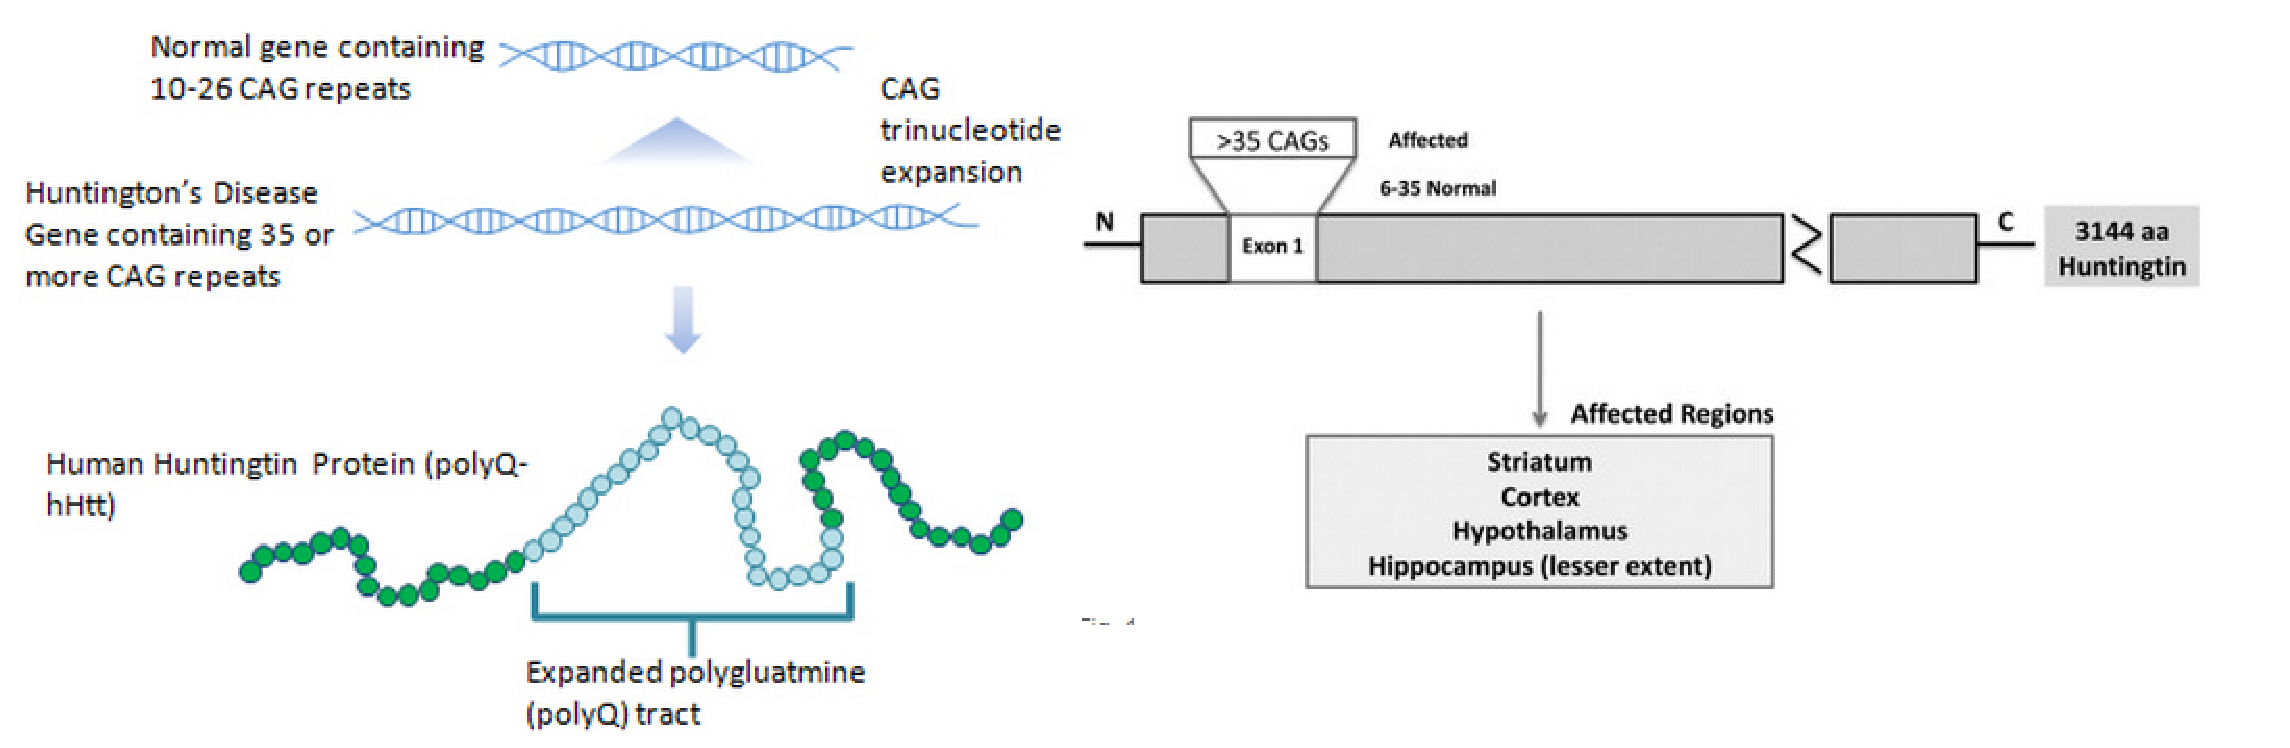
\includegraphics[height=4cm]{./images/HTT_polyQ.eps}}
  \caption{Expanded polyQ repeats within exon 1 of Huntington's disease
  gene.}\label{fig:HTT_polyQ}
  %http://www.sciencedirect.com/science/article/pii/S0925443911002493
\end{figure}

{\bf HOW IT CAUSEs THE DAMAGE?}: The aggregate structures interfere with several
crucial cellular proteins and systems, such as 
\begin{enumerate}
  \item  "kidnap" smaller proteins from their usual locations, preventing them
  from functioning normally within nerve cells
  
  \textcolor{red}{Example 1}: entangles and inhibits CREB-binding protein (also
  known as CBP), a smaller regulatory protein that is key for cell survival.
    
  \textcolor{red}{Example 2}: discrupt UPS by occupying proteasomes

{\bf Ubiquitin-Proteasome System} (UPS) is a quality control system -
 protein-chaperone system which tags misfolded or damaged proteins for
 re-folding, or more commonly, for degradation. A recent study 
{\small 
\begin{verbatim}
The fluorescent GFP which can detect Htt protein only in intact forms.
Fluorescence was higher in cells containing aggregates than in cells without,
suggesting that protein aggregation led to the UPS disruption.
\end{verbatim}
}
showed that Htt protein aggregates  impair UPS function, i.e. a possible
explanation for how these huntingtin bundles can lead to the death of neurons.
{\bf BUT HOW?} - the level of ubiquitin protein is normal, suggesting another
component of UPS, the proteasomes ({\it whose function is to break down protein
tagged by ubiquitin}), was affected. Protein aggregates may occupy the
proteasomes, inhibiting their normal activity.
 \url{http://web.stanford.edu/group/hopes/cgi-bin/hopes_test/huntingtin-protein-and-protein-aggregation/}


  \item {\bf affect axonal transport}: Normal axonal transport of organelles,
  including mitochondria, synaptic vesicles, and proteins, is essential for
  synaptic activities and neural communication.
  
%   (1) of Htt protein
%   , (2) of mitochondria
  
  \textcolor{red}{Example 1}: transport of Htt protein aggregate
  \citep{gunawardena2003}:
  Drosophila DmHTT interacts with the molecular motor dynein, associates with
  vesicles and co-sediments with microtubules.
  DmHTT co-localizes with Brain-derived neurotrophic factor (BDNF)-containing
  vesicles (Sect.\ref{sec:BDNF}) in rat cortical neurons \citep{zala2013}
  
  \textcolor{red}{Example 2}:  The N-terminal fragment of mHtt formed aggregates
  that decreases mitochondrial axonal transport, which can be an early stage
  event in the progression of HD, even before mHtt aggregates are formed
  \citep{tian2014}.  
  
  \item {\bf mitochondrial dysfunction}: abnormal mitochondrial dynamics (i.e. increased fission and decreased fusion - Sect.\ref{sec:fission-fusion})

  \item {\bf synaptic damage}:
  has been extensively reported, but the  precise factors that cause synaptic
  degeneration are not completely understood.

  Synapses are the sites of high ATP demand, and reduced number of mitochondria
  neurites and synapses produce low ATP and cause synaptic degeneration in HD
  neurons.
  \begin{itemize}
    \item presynaptic side: reduction 1.2x in synaptophysin
    (Sect.\ref{sec:synaptophysin})
    
    \item postsynaptic side: reduction 1.3x in PSD95 (Sect.\ref{sec:PSD}).
    
  \end{itemize}
  
  \item {\bf excitotoxicity}: 
  
  \textcolor{red}{Example 1}: toxicity of glutamate (neurons are damaged or
  killed by excessive stimulation by neurotransmitters such as glutamate -
  Sect.\ref{sec:Glutamate}).
  Excessive activation of glutamate receptors by excitatory amino acids leads to
  a number of deleterious consequences, including impairment of calcium
  buffering, generation of free radicals (ROS), activation of the mitochondrial
  permeability transition and secondary excitotoxicity.
  
  
  Studies found  mainly altered conductance of the N-methyl-D-aspartate (NMDA)
  glutamate receptor subtype (i.e. high $\Ca$ conductivity) and decreased levels
  of glutamate transporters.
  
  NOTE: Blood sugars are the primary glutamate removal method from
  inter-synaptic spaces at the NMDA and AMPA receptor site. Treatment is
  administered during the acute stages of excitotoxic shock along with glutamate antagonists.
  
  \textcolor{red}{Example 2}: impairment of calcium buffering (i.e. low
  buffering) or higher $\Ca$ conductivity via NMDAR/AMPAR exposes mitochondria
  to higher Ca2+ loads compared to highly buffered cell, which increases risk
  for mitochondrial damage.
  
  \textcolor{red}{Example 3}: high $[\Ca]$postsynaptic can damage mitochondria,
  trigger mitochondrial production of reactive oxygen species (ROS). ROS inhibit
  the glutamate uptake activity of EAAT2. This leads to further increases in the
  glutamate concentration at the synapse and further rises in postsynaptic
  calcium levels (Sect.\ref{sec:Glutamate}).

  \textcolor{red}{Example 4}:  alterations in energy metabolism are well
  documented in HD patients, which might facilitate excitotoxicity.
  \citep{sanchez2008}
  
  
  \item transcriptional dysregulation: 
  
  \item energy deficits: 
 
\end{enumerate}
which all underlines neuronal dysfunction and death, particularly in cortex and
striatum.




In a recent large-scale interaction network for Htt protein,
\citep{tourette2014} identified more than 100 Htt interacting proteins (HIPs,
i.e. friends of Htt), and more than 2000 proteins that interact with HIPs (i.e.
friends of friends of Htt).


The pathology of HD is therefore associated with nuclear and cytoplasmic
aggregates. The different hypotheses sources of HD suggested
\begin{enumerate}

  \item systems for handling abnormal proteins are impaired in cells and tissues
  from Huntington's disease patients or models
  
  \item mHTT is truncated and gives rise to toxic N-terminal fragments, i.e.
  mHTT aggregate leads to nerve cell damage and toxicity
  (Sect.\ref{sec:mHTT-protein-aggregate})

  \item post-translational modifications (PTM) of mHTT influence toxicity, via
  conformational changes, aggregation propensity, cellular localisation, and
  clearance.

  \item nuclear translocation of mHtt protein enhances toxic effects of the
  protein, in part via transcription-related effects

  \item cellular metabolic pathways are impaired in samples from Huntington's
  disease patients and models  

  \item HD mutations impacting the RhoGTPase signaling pathway interfered with
  filopodia (Sect.\ref{sec:synapse-formation}) \citep{tourette2014}

  \item dysfunction of cortical input to striatum: Sect.\ref{sec:HD-theory-cortical-input}
  
  \item dysfunction of dopaminergic input to striatum:
  Sect.\ref{sec:HD-role-of-dopaminergic-input}
  
  \item Glial dysfunction - Sect.\ref{sec:HD-role-of-glial}
\end{enumerate}

Pathogenic pathways of Huntington's disease are beginning to be unravelled,
offering targets for treatments.


% Key features of Huntington's disease pathogenesis
% \begin{enumerate}
%   \item 
% 
% \end{enumerate}


\subsection{circadian rhythm}

preclinical study with R6/2 mice showed that the imposition of sleep with
alprazolam selectively improves the cognitive deficits in this model but not
motor deficits (Pallier et al., 2007).




\subsection{--++ lowering mHtt protein}
\label{sec:HD-theory-lowering-mHtt}

The idea to lower mutant huntingtin is especially appealing in Huntington's
disease (HD). So far, therapies that directly tackle the most proximal cause of
the disease, targeting mHTT itself through directed lowering strategies, cannot
circumvent this issue, given the restricted distribution of the currently
contemplated therapeutic modalities likely within the CNS.

However, there are evidences that mHtt indeed causes the disease at the early
stage of neural development; and the question is if lowering mHtt can help?

\textcolor{red}{Question 1: does mHtt protein level or mRNA level
increase/decrease?}

\textcolor{red}{Question 2a: if they increase, does reducing mHtt protein level
or mRNA level help?} (using anti-sense technique to silent the gene)
\begin{itemize}
  \item  Antisense oligonucleotides delivered to patients with amyotrophic lateral
sclerosis have been well tolerated; small RNAs administered to rodent and
nonhuman primate brain knocked down huntingtin messenger RNA (mRNA);
short-hairpin complementary DNA of microRNAs can be expressed in
adeno-associated virus to provide long-term silencing of huntingtin mRNA and
protein (Aronin, DiFiglia, 2014) .
  
\end{itemize}

\textcolor{red}{Question 2b: if they decrease, does increasing mHtt protein
level or mRNA level help?}




\subsection{interneuron hypothesis: reduced Purkinje cell densities}
\label{sec:HD-theory-cerebellar-Purkinje-cell}
\label{sec:HD-theory-interneuron}

Fast-spiking, inhibitory interneurons - prototype is the parvalbumin-positive
(PV+) basket cell - generate action potentials at high frequency and synchronize
the activity of numerous excitatory principal neurons, such as pyramidal cells,
during fast network oscillations by rhythmic inhibition. For this purpose,
fast-spiking, PV+ interneurons have unique electrophysiological characteristics
regarding action potential kinetics and ion conductances, which are associated
with high energy expenditure. Fast-spiking, PV+ interneurons are central for the
emergence of gamma oscillations (30-100 Hz) that provide a fundamental mechanism
of complex information processing during sensory perception, motor behavior and
memory formation in networks of the hippocampus and the neocortex (Kann, 2016).

Jeste et al. (1994) in a study on 17 adult cases of Huntington's disease (HD),
17 patients with other movement disorders, 17 with schizophrenia, and 23 normal
controls.

They showd that loss of large Purkinje cells (less than 50\% of mean for normal
control) - Sect.\ref{sec:Purkinjie_nerves}. This loss could not be attributed to
aging, seizures, or cause of death, nor was it merely a part of a generalized
brain atrophy. So, they claimed that it suggests that the neuronal loss in HD
may not be restricted to small and medium-size neurons.

Considering the high concentration of PGC-1$\alpha$ in the cerebellum and the
role of the cerebellum in motor coordination, this may link to PGC-1a lacking.
This is clearly link to the PGC-1a hypothesis of disruption mitochondrial
biogenesis - Sect.\ref{sec:HD-theory-PGC-1}. However, as mentioned in
Sect.\ref{sec:PGC-1}, PGC-1a  can also drive genes besides those involved in
metabolic regulation, such as calcium buffer parvalbumin, synaptic protein
synaptogamin 2 (Sect.\ref{sec:synaptogamin-2}).

\subsection{disrupt mitochondrial biogenesis: CREB, TAF4, PGC-1a}
\label{sec:HD-theory-PGC-1}
\label{sec:HD-theory-mitochondria}

This cover the hypothesis that HD is a metabolic disease.

\begin{enumerate}
  \item N-terminal mHtt protein fragments: associate with {\it Hdh} 150 knock-in
  mouse brain and this association increases with age
  
  This disrupt the normal transport of mitochondria; reduced ATP level was also
  found in the synaptosomal fraction isolated from Hdh(CAG)150 knock-in mouse
  brain.
  
  \item 
\end{enumerate}

\subsection{-- mitochondrial fission}

Cherubini et al. (2015) showed that increased mitochondrial fission in mHtt
striatal cells can be a consequence of Cdk5-mediated alterations in Drp1
subcellular distribution and activity since pharmacological or genetic
inhibition of Cdk5 (Sect.\ref{sec:CDK5}) normalizes Drp1 function ameliorating
mitochondrial fragmentation.



\subsection{-- reduce movement (axonal transport of mitochondria): dysfunction
of glycolysis}
\label{sec:HD-theory-mitochondria-transport}

{\bf IDEA (from 2003)}: Early studies on Drosophila (Guanawardena et al., 2003)
and squid axon (Szebenyi et al., 2003) showed that mHtt affect mitochondrial
axonal transport. Later, cortical neurons transfected with mutant Htt display
reduced mitochondrial trafficking specifically to cytoplasmic htt aggregates,
and the degree of movement impairment is correlated with the size of aggregates
(Chang et al., 2006). This abnormal in mitochondrialtrafficing is also found in
HD striatal neurons in the absence of aggregates (Trushina et al., 2004).
In cultured neuronal cells, GFP-23Q-208-transfected neurons tend to travel
longer distance over shorter period of time than those in
GFP-130Q-208-transfected neurons (Orr, Li, 2008).

% 27. Szebenyi G, Morfini GA, Babcock A, Gould M, Selkoe K, Stenoien DL, Young
% M, Faber PW, MacDonald ME, McPhaul MJ, Brady ST. Neuropathogenic forms of
% huntingtin and androgen receptor inhibit fast axonal transport. Neuron.
% 2003;40:41-52.
% 26. Gunawardena S, Her LS, Brusch RG, Laymon RA, Niesman IR, Gordesky-Gold B,
% Sintasath L, Bonini NM, Goldstein LS. Disruption of axonal transport by loss
% of huntingtin or expression of pathogenic polyQ proteins in Drosophila.
% Neuron.
% 2003;40:25-40 24. Chang DT, Rintoul GL, Pandipati S, Reynolds IJ. Mutant
% huntingtin aggregates impair mitochondrial movement and trafficking in
% cortical neurons.
% Neurobiol Dis. 2006;22:388-400.
% 25. Trushina E, Dyer RB, Badger JD, 2nd, Ure D, Eide L, Tran DD, Vrieze BT,
% Legendre-Guillemin V, McPherson PS, Mandavilli BS, Van Houten B, Zeitlin S,
% McNiven M, Aebersold R, Hayden M, Parisi JE, Seeberg E, Dragatsis I, Doyle K,
% Bender A, Chacko C, McMurray CT. Mutant huntingtin impairs axonal trafficking
% in mammalian neurons in vivo and in vitro. Mol Cell Biol. 2004;24:8195-8209

{\bf WHY IT MAY BE IMPORTANT TO HD PATHOGENESIS}: Poor ATP distribution in
nerve terminals is likely to be an initial outcome and can affect the cellular
processes that require mitochondria in a rapid and dynamic manner, e.g.
specific synaptic sites undergoing morphogenesis or potentiation and are likely
to actively recruit mitochondria under normal conditions.
\begin{enumerate}
  \item   reduced synaptic ATP level and impaired activity of
  ubiquitin-proteasomal system (UPS) in synapses of HD mice  (Li, Orr et al.,
  2011)

UPS function is largely dependent on ATP. Synaptic UPS may be more vulnerable to
impaired mitochondrial function or deficient ATP supplies in nerve terminals. 
  
  \item 
\end{enumerate}

\begin{mdframed}
The lengthy and highly branched neuronal processes (axons and dendrites)
constitute complex neural networks in which there is a large demand for
mitochondria-generated energy (Sect.\ref{sec:mitochondria-brain}). Thus, the
impaired mitochondria trafficking in neuronal cells
(Sect.\ref{sec:mitochondria-brain-transport}) may play an important role in the
selective neuropathology of Huntington's disease. Energy consumption in the
brain - Sect.\ref{sec:brain-resting-energetic-demand}.

\end{mdframed}

{\bf EVIDENCE OF MECHANISM}:
\begin{itemize}

  \item disrupt the binding of mitochondria to microtubule-based transport
  proteins:
  
  mHtt interact with HAP1 (in Human) or its homolog in Drosophila Milton. In
  Drosophila, Milton interacts with Miro - a mitochondrial Ca2+-binding GTPase
  (Saxton, Hollenbeck, 2012) through which it binds and control kinesin.
   
   Here, Orr, Li (2008) showed that it is the soluble N-terminal fragment, not
   the full-length protein, interferes with the transport process via
   interfering the in vitro association of microtubule-based transport proteins
   with mitochondria.
  
  \item disrupt production of ATP required:  The energy required for fast axonal
  transport (Sect.\ref{sec:fast-axonal-transport}) is those from glycolysis
  (Sect.\ref{sec:glycolysis}); and mHtt affect this process at step 6 of the
  reaction chain by inflicting GAPDH enzyme - Sect.\ref{sec:GAPDH-enzyme}.
  
  On rat cortical neurons, although inhibiting ATP production from mitochondria
  did not affect vesicles motility, pharmacological or genetic inhibition of the
  glycolytic enzyme GAPDH reduced transport in cultured neurons and in
  Drosophila larvae (Zala et al., 2013). mHtt interaction with GAPDH (the enzyme
  involves in step 6 of glycolysis - Sect.\ref{sec:GAPDH-enzyme}) (Zala et al.,
  2013) or BDNF.
  GAPDH localizes on vesicles via a huntingtin-dependent mechanism and is
  transported on fast-moving vesicles within axons.

  
\end{itemize}



\subsection{-- reduced ATP production}

{\bf IDEA}:  The idea was originally derived from clinical observations of both
peripheral weight loss and central deficits in brain glucose utilization in HD
patients (Sanberg et al., 1981; Kuhl et al., 1982). Post-mortem HD brain tissue
have consistently revealed deficits in enzymes of the mitochondrial TCA cycle
and OXPHOS system. Decreased complex II/III activity and complex II (SDH)
expression are seen in HD striatum but not cortex or cerebellum (Browne et al.,
1997; Benchoua et al., 2006).
% 14. Benchoua A, Trioulier Y, Zala D, Gaillard MC, Lefort N, Dufour N, Saudou F,
% Elalouf JM, Hirsch E, Hantraye P, Deglon N, Brouillet E. Involvement of
% mitochondrial complex II defects in neuronal death produced by N-terminus
% fragment of mutated huntingtin. Mol Biol Cell. 2006;17:1652-1663.  
% 12. Browne SE, Bowling AC, MacGarvey U, Baik MJ, Berger SC, Muqit MM, Bird ED,
% Beal MF. Oxidative damage and metabolic dysfunction in Huntington's disease:
% selective vulnerability of the basal ganglia. Ann Neurol. 1997;41:646-653  
% 9. Sanberg PR, Fibiger HC, Mark RF. Body weight and dietary factors in
% Huntington's disease patients compared with matched controls. Med J Aust.
% 1981;1:407-409 
% 10.  Kuhl DE, Phelps ME, Markham CH, Metter EJ, Riege WH, Winter J. Cerebral
% metabolism and atrophy in Huntington's disease determined by 18FDG and computed
% tomographic scan. Ann Neurol. 1982;12:425-434.  

However, there is no significant difference in ATP level found between WT and HD
knock-in mice, yet the difference is significant at 14-month-old HD knock-in
mice comapred with age-matched WT mice. One possible explaination for this
late-stage deficit is that the impaired replacement, i.e.
due to reduced transport of mito
(Sect.\ref{sec:HD-theory-mitochondria-transport}), may lead to reduced supply of
ATP in nerve terminals (measured in synaptosomes in cerebral cortex - Orr, Li,
2008) (Sec.\ref{sec:ATP-concentration}).

That mitochondrial defects may be a direct effect of mutant huntingtin stems
from studies demonstrating mitochondrial Ca+2 defects in HD material (Panov et
al. 2002, Tang et al. 2005).
Mitochondria isolated from lymphoblasts of HD patients and mitochondria isolated
from the brains of mice expressing full-length mutant huntingtin had a similar
deficit in membrane potential and depolarization in response to Ca+2 loading.
Tang et al. (2005) found that mutant huntingtin affects Ca+2 signaling, leading
to cytoplasmic Ca+2 overload by sensitizing the InsP3R1 to activation by InsP3.

Enhanced release of proapoptotic factors such as cytochrome C from mitochondria
in medium spiny neurons was speculated to lead to apoptosis and HD.
A potentially important finding is the report of a relationship between the
polyglutamine tract length and the cellular energy status (Seong et al. 2005).
\begin{enumerate}
  
  \item Though the study was not in Htt gene, they examined the ATP levels in a
  striatal cell line generated from mice carrying an expanded CAG inserted into
  the endogenous mouse Sca1 gene and found low mitochondrial ATP production and
  a decrease in the ability of the mitochondria to take up ADP
  
  \item Mitochondrial dysfunction and deregulation of transcription
  (PGC-1$\alpha$) in HD are linked
  
   Peroxisome proliferator-activated receptor gamma coactivator-1$\alpha$ is
   a transcription factor that regulates mitochondrial biogenesis and metabolic
   pathways. PGC-1$\alpha$ null mice show many signs seen in HD such as a
   movement disorder and striatal neurodegeneration (Leone et al. 2005, Lin et
   al. 2004). 
\end{enumerate}

It is suggested that the striatum isparticularly susceptible to disruption of
energy metabolism caused by lack of PGC-1a.
Cui et al. (2006) and Weydt et al. (2006) showed that PGC-1$\alpha$ dysfunction
occurs in the striatum of HD mice and patients, i.e. mHtt causes disruption of
mitochondrial function by inhibiting expression of PGC-1alpha -
Sect.\ref{sec:PGC-1}. Overexpression of PGC-1$\alpha$ reversed the effects of
mutant huntingtin in cell models and in HD mice. Probably, mHtt protein repress
transcription of PGC-1$\alpha$ directly. Weydt et al. (2006) also indicated that
mHtt protein also interferes with expression of the genes downstream of
PGC-1$\alpha$.

This is because of a reduction in the expression of a number of genes regulated.


In HD, mutant huntingtin interferes with CREB and TAF4 regulation of PGC-1a
transcription, i.e. leading to inhibition the expression of PGC-1a. 
Levels of PGC-1a are decreased in HD striatum.
When compared with normal mice,
\begin{enumerate}
  \item In HD KI mice: PGC-1a level decreased 5.6-fold in MSN isolated from HD
  KI-mice (Menalled et al. 2003); yet PGC-1a was increased by 47-fold in HD interneurons
  
  \item (STHdhQ111 - striatum with Hdh gene added poly-Q length 111): 
   PGC-1a level decreased 10-fold 
\end{enumerate}

As STHdhQ111 cells exhibit decreased cAMP level; they tested if cAMP links to
PGC-1a. They showed that using 8-bromo-cAMP, it upregulates activity of
PGC-1a reporter; and such effects is dependent upon CRE-binding sites in
PGC-1a proximal promoter - which is known critical important for PGC-1a
regulation in several tissues. Subsequently, this increases PGC-1a mRNA level.

NOTE: (HttQ17) had no significant effect on the promoter activity; while
(HttQ75) produced significant inhibition by more than 75\% compared to the
normal huntingtin.
\begin{enumerate}
  \item overexpressed of CREB: significantly reduced but not  rescue the
  inhibitory effects of mHtt on PGC-1a promoter reporter.
  
  The effect of CREB is on CRE-binding site, as no effect was found when
  CRE-binding site is mutated.
  
  \item TAF4 plays critical role in mediating mHtt effect on Sp1-drive gene
  transcription 
  
  \item co-express of CREB/TAF4 completely reverse the effect of mHtt inhibition
  on PGC-1a promoter activity
  
  This effect is dependent upon the C-terminal domain of TAF4; as the mutant at
  this site remove effect of TAF4
\end{enumerate}

This also links to reduced Purkinje cell densities hypothesis
(Sect.\ref{sec:HD-theory-cerebellar-Purkinje-cell}), as (1) high concentration
of PGC-1$\alpha$ (Sect.\ref{sec:PGC-1}) in the cerebellum and the role of the
cerebellum in motor coordination; (2) PGC-1$\alpha$$^{-/-}$ mice exhibit ataxia
and reductions in genes involved in metabolism, synaptic function, and
structural support.
Alterations in protein expression are restricted to specific neuronal
populations within the cerebellum, especially Purkinje cells, and Purkinje cell
number and firing rate are decreased in PGC-1$\alpha$$^{-/-}$ animals (Lucas et
al., 2014).


\subsection{Huntington-associated protein 1 (HAP1: HAP1A, HAP1B)}
\label{sec:HAP1}

Huntingtin-associated protein 1 (HAP1) is the first protein  (Li et al., 1995)
to be found to bind to mHtt protein (Sect.\ref{sec:mHtt-protein}) in proportion
to the number of glutamines present in the glutamine repeat region, suggesting a
possible role of HAP1 in HD pathogenesis. There are 2 subtypes: 
HAP1A and HAP1B.


{\bf HISTORY}:
\begin{enumerate}

  \item Page et al. (1998) identified HAP1 mRNA in the following forebrain
  limbic nuclei: the amygdala, nucleus accumbens, dentate gyrus, septal nuclei,
  bed nucleus of the stria terminalis, and hypothalamus. Also, HAP1 protein is
  founded in numerous areas of the cortex, including the anterior cingulate
  cortex and the limbic cortex.
  
  Page KJ, Potter L, Aronni S, Everitt BJ, Dunnett SB (May 1998). "The
  expression of Huntingtin-associated protein (HAP1) mRNA in developing,
  adult and ageing rat CNS: implications for Huntington's disease
  neuropathology". Eur. J. Neurosci. 10 (5): 1835-45.    

  
  \item Gutekunst et al., (1998), using immunogold labeling, found HAP1 and mHtt
  co-localizes to the same subcellular locations; but not with mHtt aggregates.
  
  Gutekunst CA, Li SH, Yi H, Ferrante RJ, Li XJ, Hersch SM (October 1998). "The
  cellular and subcellular localization of huntingtin-associated protein 1
  (HAP1): comparison with huntingtin in rat and human". J. Neurosci. 18 (19):
  7674-86. PMID 9742138.  


  \item Martin et al., (1999) showed that HAP1B is preferentially expressed in
  striatal neurons during cell cycle, e.g. a part in spindle orientation,
  microtubule stabilization or chromosome movement
  
%   , is localized in mitotic spindle of dividing striatal cells, and associated
%   endosomes, microtubules and vesicles in the basal forebrain and striatial
%   neurons.
  
  Martin EJ, Kim M, Velier J, Sapp E, Lee HS, Laforet G, Won L, Chase K,
  Bhide PG, Heller A, Aronin N, Difiglia M (January 1999). "Analysis of
  Huntingtin-associated protein 1 in mouse brain and immortalized striatal
  neurons". J. Comp. Neurol. 403 (4): 421-30.
\end{enumerate}


{\bf DIRECT EVIDENCES}
\begin{enumerate}
  
  \item HAP-1 protein interact with p150$^\text{Glued}$ protein -
  Sect.\ref{sec:axonal-transport} (Block-Galarza et al., 1997; Engelender et
  al., 1997; Li et al., 1995, 1998; Schroer, 1996)
  
  

  \item Tan et al. - Bezprozvanny (2003): InsP3R1-HAP1A-Htt ternary complex:
  mHtt activates IP3R in bilayers and facilitates InsP3R1-mediated intracellular
  Ca2+ release in MSN

HAP1 is required for change in basal $\Ca$ levels. 

\end{enumerate}

\subsection{impaired TrkB receptor signaling: PTEN upregulated}
\label{sec:HD-theory-impaired-TrkBR-signaling}
\label{sec:HD-theory-impaired-PTEN}

The striatum performs multiple functions including control of movement, reward,
and addiction. Brain-derived neurotrophic factor (BDNF), a member of the
neurotrophin family, is among factors that promote survival and proper function
of this neuronal population (Sect.\ref{sec:BDNF}). BDNF determines the size of
the striatum by supporting survival of the immature striatal neurons at their
origin, promotes maturation of striatal neurons, and facilitates establishment
of striatal connections during brain development (Baydyuk, Xu, 2014).

In most brain regions, such as cortex, both {\it Bdnf} mRNA and BDNF protein are
present. In contrast, in the striatum {\it Bdnf} mRNA is virtually absent,
whereas BDNF protein levels are high.
It confirmed that the striatum cannot produce BDNF but depends on it for its
proper function, abnormalities in anterograde transport and reduced gene
expression from brain regions supplying BDNF to the striatum might cause
neuronal dysfunction and striatal atrophy.


For the past decade, the striatal pathology in HD has been attributed to a
decrease in cortical BDNF delivery.
However, striatal levels of BDNF and messenger RNA (mRNA) for its receptor - the
TrkB receptor (TrkBR - Sect.\ref{sec:Trk-B}) - appeared normal in symptomatic
BACHD mice. This also was true in the Q175 knockin mouse model of HD, which
displays a similar progressive motor and physiological phenotype (Menalled et
al., 2012; Heikkinen et al., 2012).

\textcolor{red}{It is the downstream TrkBR signaling through Akt was
significantly impaired, in particular}
\begin{itemize}
  
  \item  Impaired TrkB-mediated ERK1/2 activation (member of MAPK -
  Sect.\ref{sec:MAPK}) in HD knock-in striatal cells involves
  reduced p52/ p46 Shc expression [Gines, S., Paoletti, P., and Alberch, J.
  (2010)] which are TrkBR linker proteins.
  
  However, these linkers are not necessary for TrkBR-dependent synaptic
  potentiation (Minichiello et al., 2002).
  
  \item PTEN is upregulated - Sect.\ref{sec:PTEN}: In the study by Plokin et al.
  (2014)
\end{itemize}
There is a clear deficit in the postsynaptic response of iSPNs to BDNF. TrkBR
and MAPK signaling are impaired in HD iSPNs (Plotkin et al., 2014b).

\textcolor{red}{If BDNF and TrkBRs are not altered, why is BDNF-dependent
potentiation lost in BACHD iSPNs?}
\begin{enumerate}
  \item downregulation of the TrkBR linker proteins p52/p46 Shc has been
  reported. [NOT THE MAIN FACTOR]

  A significant decrease (40\%) in p52/p46 Shc mRNA in mHtt vs. WT
  striatal cells. 
  
  NOTE: unlike p52 Shc, p46 Shc was shown to be expressed solely in the nucleus. 
  
  
  \item In addition to activating TrkBRs, BDNF also can robustly activate p75
  NTRs, albeit less potently (Bothwell, 1995; Zhang et al., 2008).
  
  In Plotkin et al. (2014) protocol: The concentration of BDNF used to
mimic synaptic release in our experiments was near the IC50
of p75NTRs.

Indeed, knockdown of p75NTR expression fully restored
BDNF-dependent synaptic potentiation in BACHD iSPNs. 
\end{enumerate}


This is linked to the enhanced activity of Kv4.2 channels via KChIP auxiliary
proteins. Using TrkBR agonist - brain derived neurotrophic factor (BDNF); in
wild-type striata, BDNF significantly decreased the association of Kv4.2
subunits with both KChIP1 and KChIP2.

However, in HD striata, BDNF did not significantly alter the association of
Kv4.2 with either KChIP.

In iSPNs from symptomatic HD mice, TrkBR signaling is impaired by aberrant
p75NTR signaling through rho-associated protein kinase (ROCK) (Plotkin et al.,
2014a). These results are consistent with the proposition that TrkBR signaling
normally leads to Kv4.2 subunit phosphorylation, which promotes the dissociation
of KChIPs and Cav3 channels, decreasing Kv4 channel opening.

\subsection{PDE10 loss}
\label{sec:HD-role-of-PDE10-loss}

Two features make PDE10 (Sect.\ref{sec:PDE10}) particularly well suited as a
biomarker for Huntington's disease. First, it is found almost exclusively in
parts of the brain where brain cells die in Huntington's disease, i.e. PDE10A is
highly expressed in the striatum by MSNs. Second, although these brain cells
normally make a lot of PDE10, they start making less and less long before they
die in Huntington' disease.

In animals, PDE10-targeting drugs improve brain cell survival and delay the
onset of Huntington's-like symptoms (Sect.\ref{sec:PDE10-function}). In the
clinic, an ongoing trial currently recruiting subjects is now testing whether
PDE10-targeting drugs improve symptoms in humans with HD.

PDE10 loss is age-dependent in both R6/2 and Q175 mouse models, suggesting
reduced PDE10 levels is the consequence of transcriptional repression.
Transcriptional repression is an essential mechanism in the precise control of
gene expression.

PDE10 loss is found accompanied with D2-receptor loss (which explains why iSPN
is damaged first). Transcriptional repression is an essential mechanism in the
precise control of gene expression.

As PDE10 affect cAMP and cGMP level, they should also be measured.
cGMP change is measured using an ELISA (Sect.\ref{sec:cGMP}), and cAMP changes
were assessed using the phosphorylation status of CREB (Sect.\ref{sec:cAMP}).


% As a biomarker, therefore, it would give information specifically about problem
% areas in the disease. 

\subsection{reduced dendritic excitability via Kv4.2 enhanced activity}

The Kv4.2 subunit is known to be phosphorylated by serine-threonine protein
kinases, like mitogen activated protein kinase (MAPK), which is activated by
TrkBR signaling (Schrader et al., 2009). Moreover, TrkBR and MAPK signaling are
impaired in HD iSPNs (Plotkin et al., 2014b).

\textcolor{red}{Both KChIP1 and KChIP2, but not KChIP3/4, robustly associated
with Kv4.2 subunits}. In striata from HD mice, the association of KChIP1 (but
not KChIP2) with Kv4.2 channels was elevated (Carrillo-Reid, Surmeier, 2017).

The binding interaction between KChIP1 and Kv4.2 is independent of calcium or
tolerates EF-hand mutations, whereas modulation of Kv4.2 kinetics is dependent
on calcium or is highly sensitive to point mutations within the EF-hand domains
 (Frank An, Rhodes, 2010).



\subsection{HDAC4, HDAC6 inhibitors}
\label{sec:HD-theory-HDAC-inhibitor}

Michal Mielcarek, Gillian Bates, and colleagues elucidate a key role for the
transcription regulator histone deactylase 4 (HDAC4) - not within the nucleus as
you might expect, but instead in the cytoplasm (review: Robinson (2013)).
\begin{itemize}
  
  \item  They found that \textcolor{red}{reducing HDAC4 by 50\% }
  (Sect.\ref{sec:HDAC4}) in a mouse model of HD {\it reduced neuronal
  dysfunction of striatal neurons} and {\it delayed loss of motor function of
  the mice}, allowing them to perform a balancing task at 12 weeks of age as
  well as untreated mice who were a month younger.

Co-labeling HDAC4 and mutant HTT using antibodies indicated that they localized
together in the cytoplasm, but not the nucleus.
This ability of the work to separate cytoplasmic pathologies from nuclear ones
is an important advance in this field.

Antibodies showed HDAC4 bound to mutant HTT in either soluble or aggregated
form; but not to WT HTT. 
It is suggested that reducing HDAC4 reduced the total burden of HTT aggregates
throughout the brain while increasing the amount of soluble HTT. This links to
the hypothesis of mHTT aggeregation in cytoplasm as the source of the disease -
Sect.\ref{sec:HD-theory-mHTT-aggregation-in-cytoplasm}.

  \item 
\end{itemize}

\subsection{Glial dysfunction}
\label{sec:HD-role-of-glial}


\subsection{-- astrocyte}

Previously, mice neonatally engrafted with human glial progenitor cells (hGPCs),
which develop brains chimeric for human astroglia and their progenitors,
exhibit substantially enhanced activity-dependent plasticity and learning.

Goldman group showed that human mHtt glia can impact disease phenotype to normal
mice, e.g. making worse motor performance; and striatl neurons in mHtt glial are
hyperexcitable. They add (at birth of mice) mutant HD-expressing human hGPCs to
their normal HTT hGPC-engrafted controls, i.e.
\begin{itemize}
  \item   neonatally xenografted with hGPCs produced from mutant HD (with 48 CAG) human
embryonic stem cells (hESCs) while the control one has unaffected hESCs (with 18
CAG).
  
  \item lentiviral transduction of astrocytebiased hGPCs derived from second
  trimester human forebrain, to generate lines of hGPCs carrying either normal
  (23 CAG) or HD (73 CAG) repeats
\end{itemize}

Conversely, normal glia can ameliorate disease phenotype in transgenic HD mice,
i.e. striatal transplation of normal glial rescues aspects of
electrophysiological and behavioral phenotype, restores interstitial $\K$
homeostasis, slow disease progression and extends survival time in R6/2 HD mice.

However, understanding the disease via glia is still challenge due to
\begin{enumerate}
  \item lack of {\it in vivo} model that permit separate interrogation of glial
  and neuronal function
  
  \item marked differences between human and rodent glia
  \begin{itemize}
    \item human astrocytes are larger and more structural complex than rodent
    glia
    
    \item 
  \end{itemize}
\end{enumerate}

NOTE: {\bf CDC44} is highly expressed by astrocyte-biased glial progenitor
cells; so CDC44 is used as a biomarker for identifying astrocytes. 

\subsection{-- oligodendrocyte}
\label{sec:oligodendrocyte-in-HD}

The effects of mutant huntingtin on the function of glial cells, in
particular oligodendrocytes, remain to be fully investigated.

There is increasing evidence of white matter abnormalities in both HD patients
and HD mouse models, suggesting that mutant huntingtin might affect
oligodendrocyte function.

Transgenic mice (PLP-htt) that express an N-terminal fragment of mutant
huntingtin exclusively in oligodendrocytes. These mice develop a tremor by 2
months of age and have locomotor and behavioral deficits, including body weight
loss, reduced lifespan, and increased seizure susceptibility compared to control
mice.

Reduced myelin sheath thickness in the striatum, as well as reduced mRNA and
protein expression of essential myelin genes, suggest that
oligodendrocyte-specfic expression of mutant huntingtin causes an age-dependent
dysregulation of myelin gene expression.

\subsection{Demyelination of white-matter in HD}
\label{sec:HD-theory-demyelination}


Cerebral white matter (WM) changes in HD have been reported in a number of
studies (for reviews see Bohanna et al. (2008) and Klöppel et al. (2009)),
mainly using MR-based diffusion weighted imaging (DWI) and diffusion tensor
imaging (DTI) (Douaud et al., 2009; Rosas et al., 2006) - Sect.\ref{sec:DTI}).

With such an increasing evidence of white matter abnormalities in both HD
patients and HD mouse models, it suggests that mutant huntingtin might affect
oligodendrocyte function (Sect.\ref{sec:oligodendrocyte-in-HD}).


 


\section{HYPOTHESIS: network disease}


It has been long known that the areas of the brain most susceptible to the
deleterious effects of this mutation are the caudate and putamen, especially
striatal medium spiny neurons.

Before the genetic cause was found, evidence of caudate atrophy by brain imaging
was a critical diagnostic finding (Folstein et al., 1986). 
However, HDis not simply a basal ganglia disorder, and also affects different
cortical areas, the substantia nigra, cerebellum, and other subcortical nuclei
(Walker, 2007).


\subsection{Basal ganglia macrocircuit}
\label{sec:HD-theory-BG-macrocircuit}

HD is characterized by extensive cell loss especially in the basal ganglia
nuclei (Sect.\ref{sec:basal-ganglia}) and cortex, with the result that the
{\bf cortico-striatal-thalamo-cortical circuit} is thought to be particularly
affected.


Despite the challenge as pointed out in Sect.\ref{sec:HD-challenge}, 
the study at circuit level is important. 


\subsection{--++ Cortico-striatal-thalamo-cortical circuit}
\label{sec:HD-role-of-cortico-striatal-thalamo-cortical-circuit}

The cortico-basal ganglia-thalamo-cortical circuit is the principal circuit
thought to be affected in HD.

HD is characterized by extensive cell loss especially in the basal ganglia
nuclei and cortex, with the result that the cortico-striatal-thalamo-cortical
circuit is thought to be particularly affected. Its basic anatomy and
connectivity is preserved across most vertebrates, from the lamprey to the
human, making investigation of this circuitry feasible in HD avian, rodent and
NHP models.




\subsection{--++ Cortricostriatal projection}
\label{sec:HD-theory-cortical-input}


The dysfunction in corticostriatal synapses may be specific to glutamatergic
input and likely presynaptic in origin (Cepeda et al., 2003).

% C. Cepeda, R.S. Hurst, C.R. Calvert, E. Hernandez-Echeagaray, O.K. Nguyen, E. Jocoy, L.J. Christian, M.A. Ariano, M.S. Levine
% Transient and progressive electrophysiological alterations in the corticostriatal pathway in a mouse model of Huntington's disease
% J. Neurosci., 23 (2003), pp. 961-969 

Because the development of involuntary movements is a prominent feature of the
HD phenotype, dysfunctional cortical input to striatum is likely to constitute a
key component of HD neuropathology. \citep{estradasancher2013}.

The principal neurons in striatum are MSNs; which cause the major death; while
the interneurons are unaffected. Also, MSNs are classified into D1-MSN (dSPN)
and D2-MSN (iSPN). Postmortem evaluation of early-stage HD brains provides
evidence for a \textcolor{red}{preferential susceptibility of iSPNs to mHTT
insult} (Albin et al., 1992; Deng et al., 2004). The GPe also appears
vulnerable, with cellular and volumetric loss equal to that of the caudate
putamen (van den Bogaard et al., 2011). In later stages of HD, this pathology
also extends to dSPNs (Deng et al., 2004).


Direct pathway SPNs (dSPNs) project predominantly to the internal globus
pallidus (GPi) and the substantia nigra pars reticulata (SNr). iSPNs and dSPNs
play complementary roles in the control of movement and action selection:
activation of iSPNs suppress unwanted movements, whereas activation of dSPNs
promotes cortical selection of particular actions (Nelson and Kreitzer, 2014).

In [adult onset] HD patients, it starts with hyperkinetic motor symptoms; while
in contrast, hypokinesic behaviors are the predominant feature of juvenile HD
(JHD) (Letort and Gonzalez-Alegre, 2013), ascribed to 'striatal failure', when
both pathways (IP and DP) are affected. One possible explanation is that the
expression of mHTT alters the pattern of communication between CPNs (cortical pyramidal neurons -
Sect.\ref{sec:pyramidal-neuron-layer-III}) HD models suggests that the
expression of mHTT alters the pattern of communication between CPNs and MSNs in
the striatum. Striatal MSNs, moreover, send information to down stream
structures that project to thalamus, which in turn projects back to cortex,
allowing for even further disruptions in cortical processing.


\subsection{DA input}
\label{sec:HD-role-of-dopaminergic-input}

It is known that there is change in DA release
(Sect.\ref{sec:HD-theory-neurotransmitter-Dopamine}).

In Huntington's disease, the selective vulnerability of neurons in the {\bf
striatum}, where the highest concentration of dopaminergic innervations exists,
suggests an important role of dopamine in the pathogenesis of this disorder
(Sect.\ref{sec:dopaminegic_neurons}).

\section{D1 and D2 MSN}
\label{sec:HD-role-of-MSN}



\section{Drug targets}
\label{sec:drug-target-Huntington}

As Htt protein involve in interactions with more than 100 different other
proteins, it is challenging to find which protein-Htt protein interaction are
relevant for the disease and which are not.

% As the Htt protein interacts with a large number of proteins, finding which
% protein-protein interaction links to HD is a challenging task.
By combining large datasets of protein-protein interactions and filtering by
brain-specific gene expression in patients with and without Huntington's
disease, the scientists narrowed potential interactors to 13 candidates,
including 7 that are known targets in Huntington's disease.

The strategy is to reduce aggregation
\begin{itemize}
  \item targetting nuclear receptors (Chap.\ref{chap:nuclear-receptors})

PPAR$\gamma$ levels were reduced both in Huntington's disease (HD) patient
lymphocytes and the R6/2 HD mouse model. Treatment of HD mice with a
PPAR$\gamma$ agonist prevented functional impairments in these mice, extended
their survival, and also normalized the reduced expression of PCG-1$\alpha$
(Chiang et al., 2010; Johri et al., 2010; Jin et al., 2013).
It is suggested that PGC-1$\alpha$ deficiency underlies the mitochondrial
dysfunction observed in HD.

  \item avoid cleavage at residue 514 N-terminal side of mutated Htt protein
  by caspases

  RATIONALE: As caspase (CASP3 and CASP6) are expected to cleave mutated HTT
  protein, and the N-terminal segments can form the aggregates, leading to
  toxicity of Huntington disease (HD); by removing this cleave site, the
  caspases cannot cleave the protein at that N-terminal site.
  
  EXPERIMENT: Caspase-6-resistant mice did show some nuclear accumulation of htt
  fragments, their appearance was delayed \citep{wellington2000}.
  \url{http://www.alzforum.org/news/research-news/unkindest-cut-caspase-6-cleavage-huntingtin-produces-killer-fragment}

	HOW?
  \begin{enumerate}
    \item Cdk5 phosphorylation of Htt protein at Ser434: reduce its cleavage by
    caspase (tested with NH2-terminal 588 amino acids (htt588) of mutant htt).
	
	FACT: Cdk5 activity is reduced in the brains of HD transgenic mice compared
	with controls. DUE TO: polyQ-expanded htt fragments reducing the interaction
	between cdk5 and its activator p35 \citep{luo2005}.
	

    \item A 23-amino acid peptide P42 part of the endogenous Htt protein:
    the protective properties of this peptide against aggregation
    \citep{arribat2014, arribat2014s}, Fig.\ref{fig:Huntington_protein-N-terminal}
    
\begin{figure}[h]
\centerline{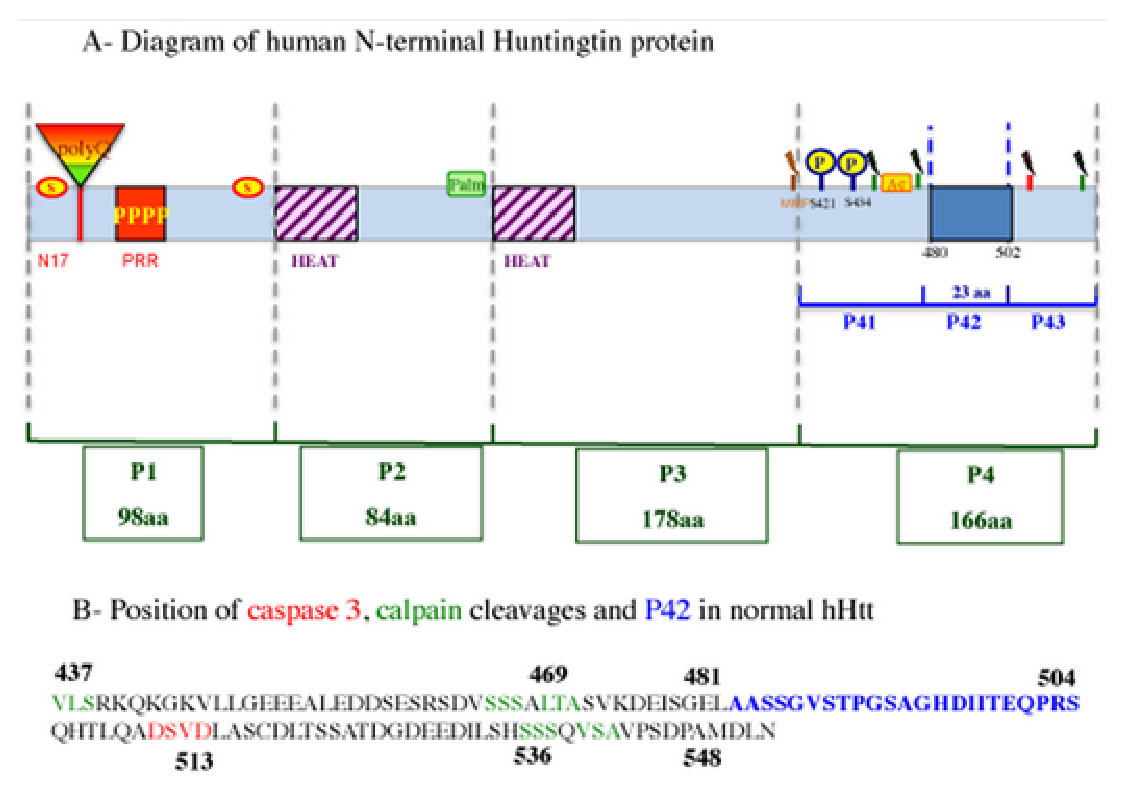
\includegraphics[height=4cm]{./images/Huntington_protein-N-terminal.eps}}
\caption{Schematic diagram of a 548
amino acid N-terminal part of human Htt protein
}\label{fig:Huntington_protein-N-terminal}
\end{figure} 
     
  \end{enumerate}
  
  \item reduce neuronal inclusion: Htt protein aggregation
  \begin{enumerate}
      \item CRMP1 gene: only express in brain:
  
  CRMP1 overexpression reduces huntingtin aggregation and cellular toxicity,
  while reduced CRMP1 results in increased aggregation and toxicity
  \url{http://genome.cshlp.org/site/press/Wanker_182444.xhtml}
  
      \item 
  \end{enumerate}   
\end{itemize}

\section{Drug: Tetrabenazine (Nitoman, Xenazine)}

Tetrabenazine is the drug name in USA (Nitoman is the name used in Canada, and
Xenazine is the name used in New Zealand and some parts of Europe) for
hyperkinetic disorders treament (not as a cure). 

Example of hyperkinetic disorder is chorea in Huntington diease (HD) - abnormal
unvoluntary movement disorder (Sect.\ref{sec:chorea})- \textcolor{red}{caused by
overactivity of the neurotransmitter dopamine in the areas of the brain that
control movement.}



\section{Zinc finger protein (ZFP)}
\label{sec:ZFP}

A {\bf zinc finger} is a small protein structural motif that is characterized by
the coordination of one or more zinc ions in order to stabilize the fold. 

Proteins that contain zinc fingers ({\bf zinc finger proteins}) are classified
into several different structural families. 
Such protein are found to be expressed from about 3\% of the genes of the human
genome.

Zinc fingers have become extremely useful in various therapeutic and research
capacities. Zinc finger proteins can bind to DNA sequence in a way to be
distinct from many other DNA-binding proteins that bind DNA through the 2-fold
symmetry of the double helix, instead zinc fingers are linked linearly in tandem
to bind nucleic acid sequences of varying lengths.

Zinc fingers proteins can be engineered to target and bind specific DNA
sequences, and enables the regulation of those genes to which they are attached.

\textcolor{red}{Application in HD}: Researchers of the Centre for Genomic
Regulation (CRG) in Barcelona designed a ZFP-targetted mHtt protein, i.e.
specificially bind to more than 35 repetitions of CAG triplet, preventing the
expression of the gene containing these repeats and reducing the production of
the mutant Huntingtin protein.


\section{*** network dynamics}	

Cepeda's data showed the number of connections between MSN in HD goes down; but
for the set of MSN pairs that form connection, they saw an increase from 0\% to
50\% of bidirectional connections between every 2 connected MSNs.

Kozloski (2010) suggested STDP eliminate loops. So, the forming of loops here
may suggest a change in STDP. The question is does STDP forms between MSNs?

In striatum, it shows winnerless network behavior. But in HD, it shows
winner-take-on in striatum (Rebec's data (2008)), like those in PFC (Miller et
al.2008).
However, the definition of burst is subjective (what constitute a burst)?

Pengsheng suggests
\begin{itemize}
  \item iSTDP
  \item homeostatic (intrinsic) plasticity
\end{itemize}
leads to healthy dynamics.

These
\begin{itemize}
  \item connectivity modification
  \item strong (cortrical excitatory) input
  \item cell death
\end{itemize}
leads to unhealthy dynamics.

Pengsheng then quantify the relationships
\begin{enumerate}
  \item fraction neuron death vs. prob. of H-neuron

Def. H-neuron: divide the time period $t$ after killing neuron into $n$ bins, if
a neuron have spiking in more than 80\% of total number of bins then it is
H-neuron.
 
Sigmoidal shape suggest neuron death is not a major factor, as 10\% lost is
still ok, but can be severe if it gets to 40\% lost.

  \item fraction of bidirectional connectivity vs. prob. of H-neuron

Network dynamics is very sensitive to bidirecitonal connection; may be a
critical factor here.
  
  \item weight of bidirectional connectivity (i.e. change in structural
  plasticity) vs.   prob.   of H-neuron
  
The weight is not that important once the bidirectional connectivity increases
to a certain value, e.g. 5\%.  It suggests that the changes in structural
plasticity (likely we all have) is harmless.

  \item topological change vs. risk-level (a neuron becoming H-neuron)
  
There are total 1000 topologies, defined based on (1) fractional bidirecitonal
connection, (2) weight values, and (3) initial configurations (i.e. number of
simulations).

Example: 20 data points, 5 different weight values, 10 simulations. So  
20x5x10 = 1000 risk levels.
\begin{itemize}

  \item high-risk neuron: sensitive to topolical change
  
  \item low-risk neuron: insensitive to topological change
\end{itemize}

\end{enumerate}


Result of Network's health recovery compared to the baseline (the one at the
botom is the best strategy). 
In normal network, increase bidirectional connection, find the H-neuron, and
modify the inputs using one of the following strategies, i.e. modifying the
plasticity rule. Each strategy reflects a line of defense. The order of
different lines of defense is given by (number) - the smallest value means the defense line occurs first.
\begin{enumerate}
  \item GABA decreases

  \item baseline
    
  \item GABA increase
  
  \item (1) GABA increase + GLT-1 increase
  
  \item (2) desensitize AMPA (DES) + GABA decrease
  
  (3) GLT-1 decreases due to cell deaths: challenge the network again
\end{enumerate}
But, still in Pengsheng's result, they are still so sensitive to bidirectional
connectivity, i.e. all give the same result (100\% H-neuron) at > 3\% of
bidirecitonal connectivity.

It's challenging to derive an STDP learning rule that can eliminate loops.
Kozloski suggested
\begin{itemize}
  \item  If post $> \theta_1$, i.e. post has been bursting for a while
  
  
  \item If $\theta_0 <$ post $< \theta_1$: 
\end{itemize}
$\Pi_\text{LTP}$ and $\Pi_\text{LTD}$.
But MSN does not expression Cannabinoid receptors, so how its synapses possess
LTD ??? However, it's worthy to know that FS interneurons (fast-spiking)
(with 5\% presence in total striatum neurons) does possess endogeneous
cannabinoid receptors.

In HD R6/2 animals, Rebec's group found very strong (and short-lived) increase 
in LFP power/amplitude; but the change is very subtle in normal mice. It
suggested the R6/2 HD mice cannot make decision due to some significant changes
in LFP. But it's very challenge to make R6/2 mice moving as they rarely move,
i.e. severe dysfunction in the motor control.



\section{*** dopaminergic neurons}

Dopaminergic neuron has very complex subthreshold oscillations: 2 types of
oscillations (BK(Ca) channels and Ca2+ concentration).
\begin{enumerate}
  \item 1
  
  \item 2
\end{enumerate}

Dopamine alters excitability of MSNs (Hopf et al. Neuroscie. 2003)

Precise timing for DA release may be crucial for cortico-striatal plasticity. 
(Yagishita et al, Science 2014). 

Tim's suggest:
DA receptor deficits and striatal DA level correlate with HD (Schwab et al.,
Exprt Rev. Neurother. 2015)

\begin{itemize}
  \item DA level increases in early stage of HD (i.e. pre-manifest)
  
  
  \item DA receptor (i.e. probably correspond to MSN level) gradually decrease
  at all stages of HD
\end{itemize}

\begin{mdframed}
A repeat of 60 CAG, and at 20 years old, and it has the same disease progression
with one at 40 years old with 30 CAG repeats for example. So, this
multiplication between age and number of CAG repeats is a better reflect of
disease progression.

\end{mdframed}


\section{*** MSN}

CHDI expects reports on STDP (LTP, LTD) on Q2-3 2016.

\section{Huntington disease-like 2 (HDL2) }
\label{sec:HDL2}
\label{sec:Huntington-disease-like-2}

Huntington disease-like 2 (HDL2) is a progressive, late onset autosomal dominant
neurodegenerative disorder, with remarkable similarities to Huntington disease (HD).
HDL2 is rare, with fewer than 50 pedigrees described worldwide
(outside of South Africa).

Unlike CAG expansion in HD (on chromosome 4p16.3 - Sect.\ref{sec:HTT_gene}),
HDL2 is caused by a CTG repeat expansion chromosome 16q24; which is the locus of
the alternatively spliced exon 2A of junctophilin-3 (JPH3). Normal alleles
contain 6 to 28 triplets, whereas pathogenic repeats range from 40 to 59.
\textcolor{red}{HDL2 with JPH-3 expansion is found in 1-15\% individual with
clinically and pathologically symptions like HD yet without HTT gene mutation.}
(Krause - Margolis, 2015; Landstrom et al., 2014).
HDL2 disease seems to be the {\bf loss-of-function} mechanism; while in HD, it
is the {\it gain-of-function}.

REMINDER: The JPH3 protein product serves to stabilize junctional membrane
complexes and regulate neuronal calcium flux (Sect.\ref{sec:JP-3}).

\begin{itemize}
  \item All patients to date with HDL2 have some African ancestry.
  
  
  \item the first mouse model of HDL2 if human BAC containing the complete JPH3
  gene with a repeat of about 120 CTG/CAG triplets and intact 30 and 50 flanking regions

  \item Jph3 null mice exhibit adult onset, progressive motor dysfunction,
  whereas Jph3 hemizygous mice have a similar but milder phenotype

This suggests that loss of JPH3 protein expression is not the sole
pathomechanism of HDL2

\end{itemize}

The molecular mechanisms underlying HDL2 remain unknown. The clinical,
neuropathological, and genetic similarities of HDL2 to HD 
\begin{enumerate}
  
  \item \sout{suggested that the HDL2 mutation would be translated into an
  expanded polyglutamine repeat (CTG $\rightarrow$ CAG repeats).}  (Wilburn et
  al., 2011)
  
  
  Seixas - Rudnicki (2012) showed no detectable changes in expansion of CAG
  triplet frontal cortex in HDL2 sample; while it can be detected in HD frontal
  cortex.

  \item loss of expression of full-length JPH-3  (Seixas et al., 2012)
  
  
  
  \item  toxic properties of JPH3 transcript containing an expanded CUG tract
  (Rudnicki et al., 2007)

  \item repeat-associated non-ATG (RAN) translation [Zu et al., 2011],
  
  RAN translation is the mechanism by which multiple homopolymeric amino
  acid-containing protein tracts may be translated on repeat disease loci.
  
\end{enumerate}





\section{p35 protein}
\label{sec:p35-protein}

p35 activates CDK5. However, its cleavaged form, p25, can also prolong CDK5
activation and changing its cellular location.

p35 form of this protein is proteolytically cleaved by calpain, generating a p25
form. The cleavage of p35 into p25 results in relocalization of the protein from
the cell periphery to nuclear and perinuclear regions.
The p25 form accumulates in the brain neurons of patients with Alzheimer's
disease. This accumulation correlates with an increase in CDK5 kinase activity,
which may lead to aberrantly phosphorylated forms of the
microtubule-associated protein tau found in AD (Sect.\ref{sec:tauopathies})

\section{p53 pathway}
\label{sec:p53-pathway}

p53, also known as TP53 or tumor protein (EC :2.7.1.37) is the gene that codes
for a protein that regulates the cell cycle (i.e. programmed cell death) and
hence functions as a tumor suppression.

Mitochondria - Sect.\ref{sec:mitochondria}

\section{Negative drug trials}

\subsection{Dietary: CREST-E with creatine}

It ends in 2014.
\url{https://nccih.nih.gov/research/extramural/crest-e}

\subsection{Dietary: 2CARE with coenzyme Q10}

CoQ10 acts to shuttle high-energy particles through the process of energy
creation.

In HD patients, we observe reduced levels of energy, almost as if the power
plants aren't working at full capacity. This suggested that, perhaps, bolstering
energy production could be a useful treatment for HD.

The trials give CoQ10 pills to HD patients.
\begin{itemize}
  \item no benefit was found on the dose and duration tested - 600 or 1,200 mg a
  day for six months in 1996.
  
  \item CARE study, treated a larger number of patients (347) for a longer time
  period (almost 3 years), found that the compound was well tolerated, but that
  it had no robust benefits in terms of HD symptoms.
  
  researchers also began reporting that high doses of CoQ10 made some HD mouse
  models better. This poses a bit of a conundrum: why would the compound make HD
  mice better, but not HD patients? 
  
  The simplest explanation is that CoQ10 simply doesn't work. Another possible
  explanation is that it might have beneficial effects in HD, but too low a dose
  had been tested. A large Parkinson's disease study, published in 2002,
  suggested that very large doses of CoQ10 (as high as 1,200 mg per day) were
  tolerated by patients with this disease. However, even though those mice that
  received the largest doses of CoQ10 seemed to do the best; in a small human
  study, published in 2010, researchers observed that human HD patients were
  able to take up to 3,600 mg a day of CoQ10 without important negative effects.

 Now we know that HD patients can take very large doses of CoQ10 and that, at
 least in mice, these large doses are the most beneficial ones.
 
 \item 2CARE study (started 2008; and was halted due to futility) tried to
 investigated large dose, intended to enroll 609 volunteers, use a very large
 dose of CoQ10 (2,400 mg a day), and treat volunteers for a whopping 5 years.

The differences between the groups (7\% vs. 4\%) could have happened by chance,
and may not have been due to the drug treatment.

Futility means pointlessness, and in the context of a clinical trial, futility
means that an interim analysis shows that the results are so unlikely to be
positive that there's no point in finishing the trial.

  
\end{itemize}
\url{https://en.hdbuzz.net/171}

\subsection{Amaryllis with PDE10 inhibitor}


The Amaryllis trial was testing am experimental drug code-named PF-02545920,
which acts on signalling chemicals inside brain cells. It had been hoped that it
would improve the communication between neurons.

PF-02545920 reduces the activity of a molecular recycling machine called
phosphodiesterase 10, so it is known as a PDE10-inhibitor.

The open-label extension study, in which everyone receives the active study drug
at the highest dose they could tolerate.
Marielle Delnomdedieu, who led the Amaryllis study for Pfizer.

The trial drug (includes 271 HD patients in 5 countries) failed to show
significant improvement in the main symptom it was targeting (i.e. primary
endpoints) – movement function – or any of the other symptoms it might have
helped with – thinking ability, behavioural problems and activities of daily
life. The trial was stopped in 2016.



\url{https://en.hdbuzz.net/229}

\section{Theurapeutic strategies}

\subsection{Gene silencing}

Huntingtin-lowering antisense oligonucleotides (ASOs) is an effort to develop a
drug that reduces levels of both the mutant and the healthy copy of the HD gene
- carried out by Roche and Ionis. The current ASO trial in humans is a
huntingtin lowering, or gene silencing therapy, which works to disable both
copies of the HD gene in short bursts. If the treatment is halted, the gene will
recover its function.
 
Some research in mice has suggested that this is harmless during later life, 
but it's difficult to be sure, because a mouse's lifespan is much shorter than
a human's. 



\subsection{Gene editing (from 2017)}

Gene editing using CRISPR-Cas9 creates a permanent change to the DNA, and
therefore must be approached with even more caution, compared to gene silencing
techniques. 
There's evidence that the HD gene, damaged or not, has important functions in
the cell, and we don't want to risk permanent side effects.

Most people with HD have only one copy of the mutant gene, and another copy that
is perfectly healthy. There is some concern about using CRISPR-Cas9 as a
therapy, because while it could delete the damaged portion from the HD gene, it
could also permanently remove a part of the healthy copy
(Sect.\ref{sec:allele}). Because of that, HD scientists are also tackling the
challenge of avoiding the healthy copy of the gene, known as an allele-specific
approach.

Whether either updated CRISPR technique will improve the behavior of an HD mouse
remains to be seen.

\begin{enumerate}
  \item  using CRISPR-Cas9 - Sect.\ref{sec:CRISPR-Cas9}
  
  What if we could edit the CAG repeat mistake, like deleting all those
  extra 'on-and-on' repeats from the previous sentence?
  
  Xiao-Jiang Li, working at Emory University in the USA, found that making tiny
cuts in the HD gene could have beneficial effects in HD mice. For these
experiments, they were using CRISPR-Cas9 in the delete mode, rather than editing
the HD gene to remove the long C-A-G with a short one.
  
  The laboratory's newest findings show improved HD mouse behavior after
  delivering CRISPR-Cas9 to the brain.
  After three months, there were fewer harmful clumps of huntingtin protein
   built up in brain cells, and the HD mice had improved somewhat on movement
   tests. The most exciting aspect of this experiment was the recovery of older
   mice that had already developed symptoms.  ven 9-month-old mice (around
   middle age) improved after receiving the injections, suggesting that their
   brains could recuperate partially after half a lifetime of damage. 
   
 \item using allele-specific CRISPR-Cas9:

Jong-Min Lee at Massachusetts General
Hospital made an allele-specific deletion using cleverly designed guide RNAs.  
  Beverly Davidson at the Children's Hospital of Philadelphia, used a similar
  approach to target only the mutant gene, making smaller cuts with Cas9
  
  
The guides sought out tiny discrepancies in the DNA letters close to the HD
  mutation and directed two Cas9 cuts. Their approach is novel because gene
  edits could be “personalized” depending on an individual's DNA.  

  
\end{enumerate}



Whether either updated CRISPR technique will improve the behavior of an HD mouse
remains to be seen


\chapter{Pre-clinical studies}

\section{What can affect pre-clinical outcomes?}

A key to reducing the variability in a mouse trial is the rigorous
standardization of the testing condition.

\begin{enumerate}
  \item  the genetics of a given HD mouse model has to be carefully
controlled

  \item If possible, an inbred mouse background should be used for a study -
  Sect.\ref{sec:mouse-inbred-background}.
  
It is not recommend that all the mouse trials for all the different types of HD
models (Sect.\ref{sec:HD-mouse-models}) should be done in the same genetic
background, although it is well known that certain behavioral readouts may be
more robust in one inbred background than another (Crawley et al. 1997).

It is recommended, however, within the same type of model, a consistent and
relatively pure genetic background (i.e., inbred or recombinant F1) should be
used, and preferably a genetic background in which a given model exhibits the
most robust phenotypes that will be used as preclinical outcomes (i.e., YAC128
model in FvB background) (Van Raamsdonk et al., 2007).

   \item mouse housing and diet conditions should also be standardized

NOTE: environmental enrichment and dietary influences, which may significantly
improve outcomes in HD mice (Hockly et al., 2002; Schilling et al., 2004a;
Spires et al., 2004). 

For R6/2 mice, a moderately enriched housing condition is recommended (Hockly et
al., 2003).
   
For other HD mouse models, such as the full-length models, the housing
conditions should be maintained constant in different trials and comparable
across different laboratories.
   
   \item the mice used in the study should be routinely genotyped to rule out
   any mice with dramatic expansion or contraction of the repeats, e.g. CAG
   repeats in HD. 

   \item the outcome testing conditions and statistical analyses should also be
   the same for a given model in different trials and different laboratories.

One challenge is that equipment and methods for behavioral testing and neuropathological
studies (i.e., stereological counting and dark neuron quantization) may be
different from laboratory to laboratory. 
  
   \item For the phenotypic studies, the investigators conducting the tests
  should be blind to the genotypes
  
   \item statistical analyses should be performed in the same way for a given
   outcome in a given model, so one can readily compare the preclinical results
   of different compounds and their ability to be replicated by different
   laboratories.
\end{enumerate}

\section{Target for pre-clinical studies in HD}

\subsection{phenotypes}

In animal models:
\begin{enumerate}
  \item  The primary phenotypic outcomes are rotarod for motor behaviors and
stereological measurement of the striatal atrophy

  \item Secondary outcomes, such as weight loss and lethality, are only
possible for the fragment models, and their relevance to HD remains unclear.
\end{enumerate}

However, in HD patients, the clinical features are far more complex and consist
of motor, psychiatric, and cognitive deficits. We are currently unclear 
\begin{enumerate}
  
  \item  whether this clinical triad is caused by neurodegeneration or neuronal
  dysfunction in HD.

  \item whether different brain regions may mediate these distinct deficits,
\end{enumerate}
the exclusive use of motor and striatal pathology outcomes (as a comparison
with those in animal models) may be insufficient, particularly in evaluating
candidates that may selectively improve cognitiveand/or psychiatricrelated
phenotypes (which may be highly relevant to HD).

Yang and Gray (2011) suggested the use of robust cognitive measures, especially
those affecting the same corticostriatal neural circuit as in patients, should
be evaluated carefully and should be included when possible as primary outcome
measures in HD preclinical studies.

\subsection{biomarkers}

Finding good biomarkers that may reflect the disease process in patient is of
particular important. Some of these potential biomarkers, such as gene
expression alterations and/or specific molecular changes in the serum such as
increase in 8-OHDG (a marker for oxidized damage to DNA), have already been
elucidated in patients (Dalrymple et al., 2007; Hersch et al., 2006; Runne et
al., 2007).

In a preclinical study with creatine, 8-OHDG was shown to dramatically normalize
with the treatment, thus indicating it may be a useful peripheral biomarker that
can predict therapeutic benefit (Hersch et al., 2006).

If similar biomarkers also are altered in preclinical mouse models, they could
be incorporated in the mouse trial to provide the opportunity to noninvasively
monitor preclinical outcomes in mice and clinical outcomes in patients.

\section{Potential drug compounds}

With the predominant use of fragment models of HD, a large set of compounds have
already been demonstrated to have preclinical efficacy (Beal and Ferrante,
2004). 

Several of these compounds, including creatine, coenzyme Q, $\alpha$-lipoic acid,
cystamine, and histone deacetylase inhibitors, have been consistently beneficial
in multiple HD mouse models and in trials done by different laboratories (Beal
and Ferrante, 2004).

If the role of a genetic mouse model in a rational development of therapy for HD
or other brain disorders remains unproven, we may learn some lessons from
another field such as cancer research.

\begin{enumerate}

  \item   mouse genetic models have provided critical mechanistic insights
into the disease pathogenic process (Frese and Tuveson, 2007; Van Dyke and
Jacks, 2002);

some lessons about the difference in the biology between the mouse and human,
which allowed the building of better mouse models (Rangarajan and Weinberg,
2003); 

   \item and eventually a few success stories-in the case for acute
   promyelocytic leukemia (APL), a mouse model of APL provided promising
   preclinical results (Lallemand-Breitenbach et al., 1999), which subsequently
   translated into effective new treatment for patients (Soignet and Maslak, 2004).

\end{enumerate}


\subsection{creatine}

\subsection{coenzyme-Q}

In Phase III clinical trial demonstrated coenzyme Q10, which has reproducible
efficacy in the preclinical models of HD (i.e., R6/2 and N171-82Q mice), also
reveals a nonsignificant trend (14\%) of improvement in HD patients (NOTE:
remember it should be 33\% or more to be considered significant).



\subsection{alpha-lipoic acid}

\subsection{cystamine}

Cystamine remains the only compound that satisfies the dual-model testing
paradigm, demonstrating some efficacy in both fragment models (Beal and
Ferrante, 2004) and in the full-length YAC128 model (Van Raamsdonk et al.,
2005b).



\subsection{histone deacetylase inhibitors}

\section{HD mouse models}
\label{sec:HD-mouse-models}

A mouse model is often used to study a disease based on either knock-in (or
knock-out) or transgenic (i.e. random integration) - Sect.\ref{sec:mouse-model-HD-Huntington}.
\textcolor{red}{Currently, we do NOT have a so-called 'right' animal model for
HD.} The available animal model can replicate some of the symptoms, but not
necessary truly capture the effective cause of the pathogenesis of the HD.
In mouse models for HD, different mouse models show different degrees of
phenotypical similarity to the human patient.

\begin{mdframed}
These differences in phenotypic expression may be attributable to the influences
of protein context, mouse strain and a difference in regulatory sequences
between the mouse Htt and human HTT genes (Sect.\ref{sec:Htt-protein}).

Though with similarity in brain anatomy, mouse's short life span ($\approx$ 2
years) is a serious limitation for understanding late-onset neurodegenerative
disease.

\end{mdframed}

Human HTT protein (\verb!NP_002102!) is 3144 amino acids long and the mouse
protein (\verb!NP_034544!) contains 3120 amino acids, i.e. 91\% identical and
95\% similar. The human HD gene is comprised of 67 exons, but the polymorphic
CAG region that encodes the polyglutamine moiety in the huntingtin protein is
contained within exon 1.  

In general, mouse lines that contain a truncated form of the HD gene tend to
show abnormal symptoms before lines containing full-length huntingtin (
Menalled and Chesselet, 2002).

Mouse models expressing full-length versions of huntingtin have also been
created, both as transgenics (Hodgson et al., 1999; Reddy et al., 1998 ;  Slow
et al., 2003) and as knock-in models in which extra CAG repeats are inserted
into the endogenous mouse locus (Menalled et al., 2002; Shelbourne et al., 1999
; Wheeler et al., 2000).   
 
\begin{enumerate}
  \item transgenic mouse model
  \begin{enumerate}
  \item R6 lines: R6/1 and R6/2: R6 mouse lines were created with up to 150 repeats. 
  
  R6/2 - Sect.\ref{sec:mouse-R6/2}: the exon-1 (of expanded CAG) is inserted
  into the Hdh gene (the homologue of human Htt in mouse).
  
  \item  N171-82Q transgenic mouse: longer transgene than was used in the R6
  lines
  
  
  \item YAC (Sect.\ref{sec:mouse-YAC}) or BAC
  (Sect.\ref{sec:mouse-BAC}): the full-length of the human Htt gene (with
  expanded CAG) is inserted into the mouse using either yeast or bacteria.
  \end{enumerate}
  
  
  \item Knock-in mouse model
  \begin{enumerate}
    \item  Q175 - Sect.\ref{sec:mouse-Q175} 
  \end{enumerate}
\end{enumerate}

\textcolor{red}{Because of the rich repertoire of HD mouse models available, a
critical first question is which mouse model or models should be used in a
preclinical study of a therapeutic candidate?}
An ideal HD mouse model should have
\begin{enumerate}
  \item a genetic construct that is similar if not identical to the
  (human) patients

  \item robust behavioral deficits and selective neuropathology mimicking the
  patients

  \item these phenotypes are early onset, rapidly progressing, easily
  quantifiable, and have limited variablity between mice
  
\end{enumerate}
Currently, each of the current models only partially satisfies such
requirements.

\subsection{Transegic fragmented mHtt}
\label{sec:HD-mouse-model-fragment-mHtt}

mhtt fragment transgenic models exhibit early-onset and rapidly progressing
behavioral and neuropathological phenotypes associated with significant weight
loss and premature death.

These models also exhibit distinct molecular changes (i.e., gene expression
changes and 8-OHDG level) that are also replicated in the patients. However,
there is no neuronal loss observed.

\begin{mdframed}

fragment models (i.e., R6/2) have very rapid onset and progression of disease,
as well as low phenotypic variability (10-20 per treatment group in preclinical
trials); weight loss and early lethality. 

BUT: (1) neuropathology in the fragment models is more widespread and relatively
nonselective; (2) because the disease progression in patients is usually very
slow, another concern is that a potential efficacious therapeutic mechanism or
candidate in human HD (i.e., with a more slowly progressing disease process) may
not be effective in the fragment model; (3) the fragment models only express a
small portion of mhtt regulatory elements and proteins; thus, potential
pathogenic interventions requiring the intact mhtt genomic context (i.e., RNA
interference based on the full-length human htt mRNA) or the protein context
(i.e., proteolysis inhibition) could not be tested in such a model.

YET: R6/2 HD mouse model is good to test early stage therapeutic screen with
primary outcomes focusing on behavioral improvements (i.e., rotarod and grip
strength) and neuroprotection (i.e., striatal atrophy), can provide relatively
rapid information on the potential therapeutic efficacy of a large number of
preclinical candidates at a reasonable cost.
If sucessfull, then we can move on to the next step with full-length mHtt mouse
models: transgenic or Knock-in; or go directly to clinical study.


\end{mdframed}
\subsection{-- R6 lines: R6/1, R6/2}

R6 mice model was first introduced in 1996 (Mangiarini et al., 1996).
\begin{itemize}
  \item  R6 mice displayed an abnormal phenotype that was, in many respects,
  reminiscent of human Huntington's disease. R6 mice appear normal at birth, but then develop
progressive problems in movement as well as defects in learning and memory (
Carter et al., 1999; Lione et al., 1999 ;  Mangiarini et al., 1996).  
  \item In addition, R6 mice lose brain weight and body weight, which is again
reminiscent of human patients with HD (Mangiarini et al., 1996).
\end{itemize}

However, there were apparently normal numbers of striatal neurons and no clearly
degenerating neurons were seen, i.e. no cell death. Only a subset of neurons
that undergo so-called dark cell degeneration, but these cells are not numerous
and they are most detectable in the anterior cingulate (Turmaine et al., 2000).
So, while some degenerating neurons have been detected in these mice, it is fair
to say that widespread neuronal death as observed in human HD patients is not a
predominant neuropathological feature of R6 transgenic mice.
So, the usage of R6 lines were put in the center the controversy between
neuronal death versus neuronal dysfunction.

\subsection{---- R6/1}
\label{sec:mouse-R6/1}

R6/1 expresses 31\% of endogeneous Htt 
\begin{enumerate}
  \item early stage : 3 month-old
  \item advances stage: 7 month-old
\end{enumerate}

\subsection{---- R6/2}
\label{sec:mouse-R6/2}

R6/2 mice carry about 1 kilobase (kb) of human huntingtin promoter, which drives
the expression of mHtt exon-1 with about 150 CAG repeats [NOTE: Because of the
heterogeinity in the technique, the R6/2 mice can express any number in the
range 100 to 300 repeats (this is one of the reason making hard to compare data
collected from this mouse line in different labs)].
Besides, R6/2 mice also carry about 262 base pair (bp) of human Htt intron 1
sequence after the exon-1.

So, mHtt-exon-1 transgene has about 75\% of endogeneous Hdh level
\begin{enumerate}
  
  \item early stage - pre-symptomatic (i.e. motor deficit like decreased running
  wheel activities): 40 day-old (about 4.5 weeks)
  
Tests:  running wheel activities in mice individually housed, climbing a wired
cylinder, and hypoactivity in the open field test (Hickey et al., 2005).

Other observed phenotypes: including changes in circadian rhythms (Morton et
al., 2005), clasping (a dystonic posture when the mice were suspended by the
tail), tremor, involuntary jerky movements, and seizures (Li et al., 2005;
Mangiarini et al., 1996).
  
  \item intermediate: Cognitive deficits, and also psychiatrically related
  deficits.
  
HD patients exhibit perseverance of learned tasks indicating frontal-striatal
inhibition deficits (Aron et al, 2003)

R6/2 mice also demonstrate difficulty in reversing prelearned tasks in the
two-choice swim tank, T maze (Lione et al., 1999), and an automated video-based
reversal task (Morton et al., 2006).

R6/2 mice also exhibit deficits in spatial learning in the Morris water-maze
task (Murphy et al., 2000) and in contextual fear conditioning (Bolivar et al.,
2003).

Psychiatrically related deficits, R6/2 mice exhibit impairment in PPI, a
sensorimotor gating abnormality also seen in the HD patients (Swerdlow et al.,
1995) and in patients with schizophrenia (Swerdlow et al., 1994).

  \item advances stage (symptomatic): 3 month-old (or 90 days)
  
At 7-8 weeks: grip strength and rotarod deficits can be readily detected, and
these deficits increase until the animal's premature death around 16 weeks of
age
  
  \item die: 13-16 weeks 
\end{enumerate}


R6/2 mice died at 12 weeks of age (~ 3 months or 90 days), at which time, their
brains were significantly atrophied. R6/2 mice demonstrate robust brain atrophy
(about 20\% brain weight loss at 12 weeks). Striatal atrophy in these mice can
be readily measured using unbiased stereology (Li et al., 2005).

R6/2 model of HD has severely disrupted serotonergic and dopaminergic systems
(Sect.\ref{sec:HD-theory-neurotransmitter}).


%They study: Normal vs. Presymptomatic (40days) vs. Symptomatic (90 days).

Mice at 40 days do not display an overt behavioral phenotype, although subtle
behavioral changes have been observed (Lione et al. 1999). Mice at 90 days
display a marked behavioral phenotype (Carter et al. 1999).

\begin{enumerate}
  \item Klapstein et al. (2001): 
 
Presymptomatic: : lower rheobase, increase Rn (neuronal input resistance)

Symptomatic:
\begin{itemize}
  \item  morphological change: show less spine densities; smaller
  diameter of dendritic shafts, smaller dendritic field
  
  \item electrophysiological change: depolarized Vrest, decreased membrane time
  constant, alter AP; increase stimulus intensities is required to evoke EPSP
  (EXPLAIN: ??? ). Also, EPSP has slower rise time, and does not decay back to
  baseline by 45ms (possibly more open of NMDAR?)
  
\end{itemize}

Both: reduced paired pulse facilitation
   
  \item 
\end{enumerate}

\subsection{-- N171-82Q}
\label{sec:mouse-N171-82Q}


The N171-82Q transgenic mouse contains a truncated human HD gene under the
control of the mouse prion promoter, with a longer transgene than was used in
the R6 lines.

N171-82Q mice express a transprotein of 82 poly-Q and the first 171 amino acids
in the N-terminal of Hdh, show an abnormal neurological phenotype, accumulate
ubiquitinated inclusions, and have shortened lifespan, although they survive
longer than R6 mice.

\begin{itemize}
  \item symptomatic: 12 weeks
  
progressive {\bf motor deficits}: including tremors, uncoordination,
hypoactivity, abnormal gait, and clasping (Schilling et al., 1999).

Test: rotarod impairment, beginning at approximately 11 weeks of age (Andreassen
et al., 2001; Schilling et al., 2004b)

{\bf behavioral deficits}: more variable compared with R6/2 mice; thus, to
attain adequate statistical power, a typical preclinical study with N171-82Q mice would
require a large number of mice (i.e., minimum of 20) than a study with R6/2
(Hersch and Ferrante, 2004).

  \item premature death: 5-6 months (longer than R6/2)
\end{itemize}



\subsection{-- HD94}
\label{sec:mouse-HD94}

HD94 is another line of exon1 mice, but in this case, the transgene, which has
94 glutamines, is tetracycline-regulatable ( Yamamoto et al., 2000)

In HD94 mice, turning off transgene expression resulted in reversal of
neuropathological and behavioral measures, suggesting that some of the pathology
in HD is potentially reversible. 


\subsection{Transgenic full-length mHtt}
\label{sec:HD-mouse-model-full-length-mHtt-transgenic}
The advantage of full-length Hdh-KI (fl-mhtt Tg) and mhtt transgenic models
is that they may better resemble the pathogenic mechanisms that occur in the
patients (Gusella and MacDonald, 2006; Van Raamsdonk et al., 2007).

The shared disadvantage of these models, compared with the fragment models, is
that they are slowly progressive models, and quantifiable motor and pathological
deficits usually do not occur until 6-12 months of age.

The human fl-mhtt Tg mice, BACHD and YAC128, both exhibit progressive rotarod
and open field deficits, late onset, and selective neuropathology reminiscent of
HD. In these two models, rotarod deficits and striatal or cortical
atrophy may be used as outcome measures in a preclinical study. In the next
section, we will discuss how these HD mouse models can be used for preclinical
studies in HD.

\begin{mdframed}

The full-length mHtt models have advantages: 
(1) have genetic, genomic, and protein context more similar to human HD; (2)
have a slowly progressing disease process that may be more closely related to
the process in the human disease; and (3) have neuropathology that is selective
to the striatum and cortex. 

However, the main concern in the use of the full-length models in preclinical
trials is cost, which is relatively high because of the length of the trial
(i.e., up to 12 months in YAC128 and BACHD mice and up to 1-2 years in Hdh-KI
mice), as well as because of the potential variability of their outcomes, which
may require a larger number of mice for each study (see below). However, recent
studies using YAC128 mice in preclinical studies provide some examples of
full-length models being effectively used to identify promising preclinical
candidates in HD (Van Raamsdonk et al., 2005b, 2005d).

To save cost, a preclinical study using fragmented mouse models can be a good
option (Sect.\ref{sec:HD-mouse-model-fragment-mHtt}) However, that step is not
necessary if (1) the mechanism of therapy requires the genomic or protein
context of the full-length mhtt (i.e., small interfering RNA against human
full-length mRNA, or proteolysis inhibitor targeting mhtt regions beyond those
in the fragment models); or (2) the therapeutic modality favors a more slowly
progressive and/or selective disease process (i.e., aging-related therapeutic
targets).

Nevertheless, the dual-model approach in which first screening with a fragment
model of HD and then following up with a second study using a full-length model
is the most rational and prudent approach to identify promising clinical
candidates in HD.

\end{mdframed}

\subsection{-- YAC128}

\subsection{-- BACHD}

\subsection{Knock-in full-length mHtt}
\label{sec:HD-mouse-model-full-length-mHtt-Knock-in}

Hdk-KI mice have the advantages found in full-length transgenic mouse models
(Sect.\ref{sec:HD-mouse-model-full-length-mHtt-transgenic}).
Hdk-KI mice are the most precise genetic model of HD (i.e. we can know exact CAG
repeat numbers) and hence are valuable to study molecular mechanisms and
therapeutic interventions requiring such precise level of mutant Hdh expression
in the endogenous genomic context.

The motor and pathological phenotypes of the Hdh-KI mice are slowly progressing
and mild, but recent studies of CAG140 (Menalled et al., 2003) and Hdh(CAG)150
(Heng et al., 2007; Woodman et al., 2007) mice demonstrate that these models may exhibit
motor and striatal atrophy phenotypes that are relatively robust and could be
used as preclinical outcomes.

\subsection{-- HdhQ111}

The strongest in the 150 CAG homozygotes (Heng et al., 2007), i.e. relatively
robust display of motor and striatal atrophy phenotypes


\subsection{-- CAG140}

\subsection{-- Hdh(CAG)150}

\subsection{-- Q175}
\label{sec:mouse-Q175}


\section{Power analysis: sample size for preclinical study}
\label{sec:power-analaysis}

A very important consideration in the design of preclinical trials is to perform
power analyses for a given preclinical outcome to determine the number of HD
mice needed for a given set of outcomes in a preclinical trial (Bates and
Hockly, 2003).

Similar to the human clinical trials, insufficiently powered studies can be costly and may not provide
the necessary information to assess the efficacy of a compound. 

The question is : {\bf how many animals will be needed in a study to have a
predetermined reasonable chance} (i.e., 80\% or 90\%) of detecting a significant
improvement at a predetermined magnitude of improvement (i.e., 30\%
improvement). The basic formula for sample size estimation is the following
(adapted from Hockly et al., 2003):

The number of mice needed $n$ (in each treatment group: one control, and one
test) is
\begin{equation}
n = \frac{(\text{SD}_1^2 + \text{SD}_2^2) \times (y + z)^2  }{(\mu_1 - \mu_2)^2}
\end{equation}
\begin{itemize}
  \item $\mu_1, \mu_2$ : the mean outcomes of two groups
  
  \item SD1, SD2 : the standard-deviation of two groups
  
  \item NOTE: $y=1.96$ for p-value = 0.05 (two-sided normal distribution)
  
  \item NOTE: $z=1.28$ for power of 90\%; and $z=0.84$ for power of 80\%.
\end{itemize}

RESULT:
\begin{enumerate}
  \item R6/2 mice normally requires only about 10 mice per group for most of the phenotypic
outcomes,

  \item use of N171-82Q mice may require 20 mice per group (Hersch and Ferrante,
  2004). 
  
  \item YAC128 model, striatal atrophy is a particularly good readout because
  only 8 animals per group are needed to provide 80\% power to detect a
  significant (P < 0.05) treatment benefit that is 33\% or greater (Slow et al.,
  2003).

  \item BACHD model: the rotarod deficit at 6 months is a particularly robust
  phenotype outcome: only 22 BACHD mice are needed per group to provide 80\%
  power to detect significant (P < 0.05) improvement of 33\% or better - from
  (Gray et al., 2008) and an independent analysis at PsychoGenics (Tarrytown,
  NY) (L. Menalled and D. Howland, personal communications with Yang and Gray)
  (Yang, Gray, 2011)
\end{enumerate}




\section{Genetic background of mice: inbred mouse background vs. recombinant F1
 background}
 
A strain's genetic background profoundly affects the phenotypes that their
mutant and transgenic mice manifest.
Knowing on which strain background your mutant mice are is critical not only for
choosing the proper wild-type control strains for your experiments, but also for
comparing data between mice that carry different mutations and for comparing
data reported by other researchers for the same mutant strain.

If you don't know the strain background, you can choose a technique such as
Genome scanning. {\bf Genome scanning} is mainly used to determine the genetic
background of a strain.
Genome Scanning is based on the analysis fully customizable panel of 150-200
informative polymorphic SNPs of single nucleotide polymorphisms (SNPs). Each
marker is selectively chosen so it is polymorphic between two specific inbred
strains. Therefore each marker is informative.
\footnote{\url{https://www.jax.org/news-and-insights/jax-blog/2013/march/how-can-i-confirm-the-genetic-background-of-my-mice}}


Example: R6/2, which can only be maintained in a mixed F1 background, one should
consistently split transgenic littermates between the treatment group and
control group, and use litters from different breeding pairs to avoid potential
breeder effects (Hockly et al., 2003).


\subsection{FvB background}

\subsection{inbred background}

\subsection{recombinant F1 background}




 
 
\section{Rodents: Mouse model vs. Rat model}

Compared to other animals, such as non-human primates, zebrafish, fruit flies
and roundworms, rats and mice have been the leading model organisms used in
biomedical research. Table.\ref{tab:mice-rat-human} shows this comparison
between mice, rat and an average adult human.

Nowadays, mice rapidly overtaking rats as the major model of choice in
biological research. Along with that, rodent-based research has taken place.

Based on a large body of evidence, rats are not simply 'big mice' and, although
similar in many aspects, there are fundamental differences between these
rodents (review: Ellenbroek, Youn, 2016).
\begin{itemize}
  \item  rats have a number of clear advantages, such as the relatively large
  size of their brains, which makes brain surgery much easier 
  
  \item rats are much easier to handle than mice and less easily stressed by
  human contact
  
  \item 
\end{itemize}


\begin{table}[hbt]
\begin{center}
    \begin{tabular}{p{5cm}ccc}
        \hline
        & rat &  mice & human \\
        \hline \hline
tracer mass injected (maximal receptor occupancy of 1\%)
e.g. PET ligand for D2-receptor &  5.2 MBq & 0.3 MBq & \\
injection volume (less than 10\% of animal's 
total blood volume) & 30 mL & 2.5 mL & \\
weight & 300g & 25g & 75 kg (average-sized adult) \\
weight-scale down & 250 & 3,000 & 1 \\
size-scale down & 6 & 15 & 1  \\
        \hline
    \end{tabular}
\end{center}
\caption{Compare rat vs. mice vs. human}
\label{tab:mice-rat-human}
\end{table}


\subsection{mouse models}
\label{sec:mouse-models}

Neuroscience-related researches
\begin{itemize}
  \item using mice from about 20\% in the 1970s and 1980s to around 50\%.
  
  This is because the availability of  techniques for genetic manipulation of
  mice.
  
  \item 
\end{itemize}

The first knockout mouse was in 1987 (Thomas and Capecchi, 1987).

\subsection{rat models}
\label{sec:rat-models}

The genetic toolbox for rats is now rapidly filling up, with the introduction of
N-ethyl-N-nitrosourea (ENU) mutagenesis (Zan et al., 2003), zinc-finger
nucleases (Geurts et al., 2010), homologous recombination (Tong et al., 2011)
and, most recently, clustered regularly interspaced short palindromic repeats
(CRISPR)/Cas-mediated genome editing (Shao et al., 2014).

The whole genome of the rat was completed more than a decade ago (Gibbs et al.,
2004) and ongoing functional annotation of the genome (data are collected,
consolidated and integrated at the Rat Genome Database; see Shimoyama et al.,
2016).

\subsection{HD-pigs (from Jul, 2018)}
\label{sec:HD-pigs}

Li lab from Emory University and another one from Jinan University's
Guangdong-Hongkong-Macau Institute of CNS Regeneration have generated a genetic
model of HD in pigs using two very cool techniques which rely on genome editing,
e.g. CRISP-Cas9 (Sect.\ref{sec:CRISPR-Cas9}) to introduce a segment of human
mHtt gene  into pig fibroblast cells. Then somatic cell nuclear transfer
generated pig embryos carrying this genetic alteration. This is a {\bf Knock-in}
pig, i.e. changed gene is in its natural context.
\url{https://www.sciencedaily.com/releases/2018/03/180329141047.htm}

The truly exciting result of this new work was that the pigs themselves had very
dramatic symptoms, which appeared to mimic what's seen in human HD patients much
more closely than in rodents. The movement abnormalities, or chorea, that
patients experience was replicated as the pigs developed walking and running
difficulties with age.
They show respiratory difficulties, which resemble those experienced by humans
with HD and are not seen in mouse models of HD.  In addition, the pigs show
degeneration of the striatum, the region of the brain most affected by HD in
humans, more than other regions of the brain. 

The early results from the pig HD model  suggests large animal models could
better model other neurodegenerative diseases, such as Alzheimer's, Parkinson's and ALS
(amyotrophic lateral sclerosis).


\url{https://en.hdbuzz.net/260}

increased animal size, comes increased costs in terms of housing and feeding,
plus it takes longer for the animals to develop and reach adulthood which could
really hinder how quickly new discoveries are made. 



\section{Cre-Lox, TeT (Tetracycline), Flt-FRT, ER}
\label{sec:Cre-Lox}
\label{sec:Tet-system}
\label{sec:Flt-FRT}

The {\bf Cre} protein was purified in 1983.

{\bf Cre recombinase} (38 kDa): The enzyme plays important roles in the life
cycle of the P1 Bacteriophage. Cre recombinase is a widely used tool in the
field of molecular biology.

Cre-Lox system: the Cre enzyme is expressed on the target organism, and 
\begin{itemize}
  \item  it is used to manipulate genes and chromosomes, e.g. gene knock-out,
  knock-in. 
  
  The enzyme's ability to operate efficiently in a wide range of cellular
  environments (including mammals, plants, bacteria, and yeast) enables the
  Cre-Lox recombination system.
\end{itemize}
Joe Tsien pioneered Cre-loxP-mediated brain subregion- and cell type-specific
genetic techniques in 1996,[4] enabling researchers to manipulate or introduce
any gene in a specific brain region or a given type of neuron. 
\url{https://en.wikipedia.org/wiki/Joe_Z._Tsien}

In the Cre and FRT systems, activation or knockout of the gene is irreversible
once recombination is accomplished, whereas, in Tet and ER systems, it is reversible.
Tetracycline-Controlled Transcriptional Activation is a method of inducible gene
expression where transcription is reversibly turned on or off in the presence of
the antibiotic tetracycline or one of its derivatives.

The Tet system has very tight control on expression, whereas ER system is
somewhat leaky.
\url{https://en.wikipedia.org/wiki/Tetracycline-controlled_transcriptional_activation}

  2 elements of Tet system: (1)  the transcriptional transactivator tTA
  (tetracycline transactivator) is under the control of a cell-specific
  promoter; (2) the gene necessary to affect the target neuronal population is
  under the control of the TRE (tetracycline-responsive element) promoter that
  binds tTA and will be, therefore, regulated by the presence or absence of
  tetracycline (Gossen and Bujard, 2002).


Flp-FRT recombination is a site-directed recombination technology, increasingly
used to manipulate an organism's DNA under controlled conditions in vivo. It is
analogous to Cre-lox recombination but involves the recombination of sequences
between short flippase recognition target (FRT) sites by the recombinase
flippase(Flp)derived from the 2 $\mum$ plasmid of baker's yeast Saccharomyces
cerevisiae.

